%set the master document for easy compilation
%!TEX root = ../D3_5_3.tex

%-----------------------------------------------------------------------
\section{Manage\_TrackSideInformation\_Integration}
%-----------------------------------------------------------------------
%\tbc
%Bernd Hekele

The block ``Manage\_TrackSideInformation\_Integration'' is responsible for receiving Eurobalise telegrams and Euroradio messages from the API and perform several consistency checks on the input.

The block collects the telegrams of balises in order to build balise group messages. Euroradio messages are always delivered as a whole message. On each message, a consistency check is performed, before the data is validated according to the driving direction of the train. In general, messages not designated for the current driving direction of the train are not forwarded to the further processing. After applying consistency checks, the data direction is validated.

%Information of the odometer is used to control for the train leaving the expectation window of the balises. % TODO makes not much sense here.

\begin{figure}
 \centering
 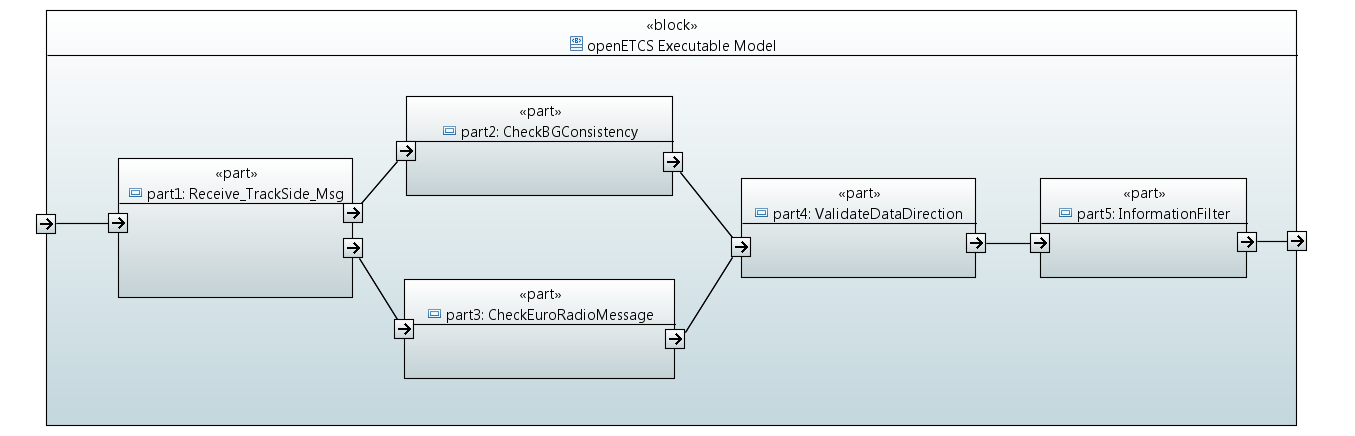
\includegraphics[width=\textwidth]{./images/Input-Messages4.PNG}
 % Input-Messages4.PNG: 0x0 pixel, 0dpi, nanxnan cm, bb=
 \caption{Structure of the Manage\_TrackSideInformation\_Integration module with submodules.}
 \label{fig:receiveAndCheckConsistencyArch}
\end{figure}


\subsection{Inputs}
For providing the output, the module needs different input data flows. An overview is provided in table \ref{tbl:ReceiveMessageAndCheckConsistencyInput}.

\begin{minipage}{\textwidth}
  \tiny
  \begin{tabular}{| c | l | l | l | l |}
    \hline
    \textbf{Index} & \textbf{Input name} & \textbf{Input type} & \textbf{Source}\\ \hline
    0 & \texttt{fullChecks} & \texttt{bool} & Configuration \\
    1 & \texttt{API\_trackSide\_Message} & \texttt{API\_Msg\_Pkg::API\_TrackSideInput\_T} & API\\
    2 & \texttt{ActualOdometry} & \texttt{Obu\_BasicTypes\_Pkg::odometry\_T} & Odometer\\
    3 & \texttt{reset} & \texttt{bool} & Environment\\
    4 & \texttt{trainPosition} & \texttt{TrainPosition\_Types\_Pck::trainPosition\_T} & Calculate Train Position\\
    5 & \texttt{modeAndLevel} & \texttt{BG\_Types\_Pkg::ModeAndLevelStatus\_T} & Mode and Level\\
    6 & \texttt{tNvContact} & \texttt{Obu\_BasicTypes\_Pkg::T\_internal\_Type} & Database\\
    7 & \texttt{lastRelevantEventTimestamp} & \texttt{Obu\_BasicTypes\_Pkg::T\_internal\_Type} & Database\\
    8 & \texttt{connectionStatus} & \texttt{Radio\_Types\_Pkg::sessionStatus\_Type} & Manage Radio Communication\\
    9 & \texttt{inSupervisingRbcId} & \texttt{int} & Database\\
    10 & \texttt{inAnnouncedBGs} & \texttt{TrainPosition\_Types\_Pck::positionedBGs\_T} & Calculate Train Position\\
    11 & \texttt{q\_nvlocacc} & \texttt{Q\_NVLOCACC} & Database\\
    \hline
  \end{tabular} 
  \captionof{table}{Overview over input}
  \label{tbl:ReceiveMessageAndCheckConsistencyInput}
\end{minipage}


\subsubsection{Input 0: \texttt{fullChecks}}
The boolean indicates, if all checks on the message should be performed. The possible values are given in table \ref{tbl:fullChecks}.

\begin{minipage}{\linewidth}
 \begin{tabular}{| l | p{9cm} |}
    \hline
    \textbf{Value} & \textbf{Interpretation}\\ \hline
    true & All checks are performed.\\
    false & The module \texttt{Information Filter} is deactivated.\\
    \hline
  \end{tabular} 
  \captionof{table}{Possible values for the input \texttt{fullChecks}}
  \label{tbl:fullChecks}
\end{minipage}

\subsubsection{Input 1: \texttt{API\_trackSide\_Message}}
The \texttt{API\_trackSide\_Message} is the message received from the API. The API performs preprocessing of RTM and BTM messages and deliveres a maximum of a single message per cycle to the SCADE model.

\subsubsection{Input 2: \texttt{ActualOdometry}}
The input \texttt{ActualOdometry} is provided by the external odometry module of the train. It contains location information with inaccuracies.

\subsubsection{Input 3: \texttt{reset}}
To delete all data stored in the module (e.g. collected balise telegrams, which do not yet form a complete message), a reset input can be used. If the input is set to \texttt{true}, all data kept in the module is deleted and no input is accepted.

\begin{minipage}{\linewidth}
   \begin{tabular}{| l | p{9cm} |}
    \hline
    \textbf{Value} & \textbf{Interpretation}\\ \hline
    true & All data kept in the module is deleted and no input is accepted.\\
    false & No action. Data at input is accepted.\\
    \hline
  \end{tabular} 
  \captionof{table}{Possible values for the input \texttt{reset}.}
  \label{tbl:reset}
\end{minipage}


\subsubsection{Input 4: \texttt{trainPosition}}
The input \texttt{trainPosition} is generated by the ``Calculate Train Position'' module and contains the current position of the train.

\subsubsection{Input 5: \texttt{modeAndLevel}}
The input is generated by the ``Mode and level management'' module. It provides the current level and mode of the EVC.

\subsubsection{Input 6: \texttt{tNvContact}}
For monitoring the safe radio connection, the national value \texttt{T\_NVCONTACT} is needed as an input.

\subsubsection{Input 7: \texttt{lastRelevantEventTimestamp}}
For monitoring the safe radio connection, it's necessary, that the time between two packets is less than the value of \texttt{T\_NVCONTACT}.

In situations like level-changes or announced radioholes, not the timestamp of the last message is relevant for comparison, but the timestamp of the last relevant event. This can be e.g. the timestamp of the level change or the timestamp of the timestamp of the moment, when the train was passing the end of the radiohole. 

For performing this check, the timestamp of the last relevant event is provided to the model as an \texttt{T\_internal\_Type}-type.

\subsubsection{Input 8: \texttt{connectionStatus}}
The input \texttt{connectionStatus} will give information about the radio connection. This input is delivered by the session management module, not from the API. The information is needed to perform the timing check, which is depending on the connection state.

\begin{minipage}{\linewidth}
\scriptsize
  \begin{tabular}{| l | p{9cm} |}
    \hline
    \textbf{Value} & \textbf{Interpretation}\\ \hline
    DISCONNECTED & The OBU is currently not connected to a RBC.\\
    CONNECTING & The OBU is currently connecting to the RBC. Received messages belong to the process of establishing a connection.\\
    CONNECTION\_ESTABLISHED &  The connection to RBC is established.\\
    \hline
  \end{tabular} 
  \captionof{table}{Possible values for the input \texttt{connectionStatus}.}
  \label{tbl:connectionStatus}
\end{minipage}

\subsubsection{Input 9: \texttt{inSupervisingRbcId}}
For the submodule ``Information Filter'', the information is needed, which radio messages are sent by the supervising RBC. To recognize these messages, the identifier of the supervising RBC is needed.

\subsubsection{Input 10: \texttt{inAnnouncedBGs}}
This input provides information about balise groups which will be passed by the train soon. This information is generated by ``Calculate Train Position'' based on the linking information received from trackside.

\subsubsection{Input 11: \texttt{q\_nvlocacc}}
The national value determines the location accuracy and is delivered by the database.



\subsection{Outputs}
The output of the module provides the received and processed Euroradio and Eurobalise messages. The module combines messages both from Eurobalises and from Euroradio to one common dataflow.

An overview over the output dataflows is provided in table \ref{tbl:ReceiveMessageAndCheckConsistencyOutput}.

\begin{minipage}{\linewidth}
 \footnotesize
  \begin{tabular}{| c | l | l | l |}
    \hline
    \textbf{Index} & \textbf{Output name} & \textbf{Output type}\\ \hline
    0 & \texttt{outputMessage} & \texttt{Common\_Types\_Pkg::ReceivedMessage\_T}\\
    1 & \texttt{ApplyServiceBrake} & \texttt{bool}\\
    2 & \texttt{BadBAliseMessageToDMI} & \texttt{bool}\\
    3 & \texttt{errorLinkedBG} & \texttt{bool}\\
    4 & \texttt{errorUnlinkedBG} & \texttt{bool}\\
    5 & \texttt{passedBG} & \texttt{BG\_Types\_Pkg::passedBG\_T} \\
    6 & \texttt{outPositionParams} & \texttt{Common\_Types\_Pkg::PositionReportParameter\_T} \\
    7 & \texttt{outRadioManagement} & \texttt{Common\_Types\_Pkg::radioManagementMessage\_T} \\
    8 & \texttt{radioSequenceError} & \texttt{bool} \\
    9 & \texttt{radioMessageConsistencyError} & \texttt{bool} \\
    \hline
  \end{tabular} 
  \captionof{table}{Dataflow at output}
  \label{tbl:ReceiveMessageAndCheckConsistencyOutput}
\end{minipage}

\subsubsection{Output 0: \texttt{outputMessage}}
The element \texttt{outputMessage} consists of the type \texttt{ReceivedMessage\_T} combines both balise and radio messages to one common datatype. This datatype contains all variables and packets, which are possible for the given scenario.

\begin{minipage}{\linewidth}
  \tiny
  \begin{tabular}{| l | l | p{5.5cm} |}
  \hline
  \textbf{Name} & \textbf{Datatype} & \textbf{Description}\\ \hline
  \texttt{valid} & \texttt{bool} & true, if no consistency errors were detected.\\
  \texttt{source} & \texttt{Common\_Types\_Pkg::MsgSource\_T} & Defines, if this is a Euroradio or Eurobalise message.\\
  \texttt{packetMetadata} & \texttt{Common\_Types\_Pkg::Metadata\_T} & contains the metadata of the packets\\
  \texttt{radioMetadata} & \texttt{Common\_Types\_Pkg::RadioMetadata\_T} & contains the metadata of the radio specific header variables\\
  \texttt{BG\_Common\_Header} & \texttt{BG\_Types\_Pkg::BG\_Header\_T} & Header of Eurobalise message\\
  \texttt{Radio\_Common\_Header} & \texttt{Radio\_Types\_Pkg::Radio\_TrackTrain\_Header\_T} & Header of Euroradio message\\
  \texttt{packets} & Common\_Types\_Pkg::Packets\_T & Structure of packets in messages\\
  \hline
\end{tabular}
  \captionof{table}{Structure of \texttt{ReceivedMessage\_T}}
  \label{tbl:receivedMessage_structure}
\end{minipage}

The Eurobalise-common-header \texttt{BG\_Header\_T} consists of the fields visible in the SCADE-declaration. The structure corresponds to the structure defined in the SRS chapter 8.4.2.1. Some fields were removed since they are not needed anymore for further processing after building messages from separate telegrams.

The Euroradio-common-header \texttt{Radio\_TrackTrain\_Header\_T} consists of the fields visible in the SCADE declaration. The structure corresponds to the structure defined in the SRS chapter 8.4.4.6.1. The structure contains all variables required by possible \texttt{NID\_MESSAGE} values for the given scenario. Which values are valid is defined in the field \texttt{radioMetadata}.

%\textbf{TODO:} Different definition of Radio-header than in SCADE!

%\textbf{TODO:} Note on packet type definitions and implementation details (which values were not used).

%\textbf{Note:} Packet 44 not used (applications outside the ERTMS/ETCS system are not supported by this implementation).

%\textbf{TODO:} Define packets 136, 12 in SCADE.

\subsubsection{Output 1: \texttt{ApplyServiceBreak}}
The flag indicates the balise group the train just passed could not be processed correctly. The check results in the request for a service break.

\subsubsection{Output 2: \texttt{BadBaliseMessageToDMI}}
Information to be passed to the DMI to indicate the reception of a ``bad balise'' to the driver.

\subsubsection{Output 3: \texttt{errorLinkedBG}}

\begin{minipage}{\linewidth}
  \begin{tabular}{| l | p{9cm} |}
    \hline
    \textbf{Value} & \textbf{Interpretation}\\ \hline
    true & A error in a linked balise group was detected.\\
    false & No error in a linked balise group was detected.\\
    \hline
  \end{tabular} 
  \captionof{table}{Possible values for the input \texttt{errorLinkedBG}}
  \label{tbl:errorLinkedBG}
\end{minipage}

\subsubsection{Output 4: \texttt{errorUnlinkedBG}}
\begin{minipage}{\linewidth}
  \begin{tabular}{| l | p{9cm} |}
    \hline
    \textbf{Value} & \textbf{Interpretation}\\ \hline
    true & A error in an unlinked balise group was detected.\\
    false & No error in an unlinked balise group was detected.\\
    \hline
  \end{tabular} 
  \captionof{table}{Possible values for the input \texttt{errorUnlinkedBG}}
  \label{tbl:errorUnlinkedBG}
\end{minipage}

\subsubsection{Output 5: \texttt{passedBG}}
The output \texttt{passedBG} provides the received balise group message in a special format needed by the module ``Calculate train position''.

\subsubsection{Output 6: \texttt{outPositionParams}}
The output \texttt{outPositionParams} provides the parameters for the position report in a special format needed by the module ``Provide Position Report''.

\subsubsection{Output 7: \texttt{outRadioManagement}}
The output \texttt{outRadioManagement} provides the messages for radio session management in a special format needed by the module ``Management of Radio Communication''.

\subsubsection{Output 8: \texttt{radioSequenceError}}

\begin{minipage}{\linewidth}
  \begin{tabular}{| l | p{9cm} |}
    \hline
    \textbf{Value} & \textbf{Interpretation}\\ \hline
    true & A sequence error or a timeout has been detected in the radio message.\\
    false & No error in the radio message sequence was detected.\\
    \hline
  \end{tabular} 
  \captionof{table}{Possible values for the input \texttt{radioSequenceError}}
  \label{tbl:radioSequenceError}
\end{minipage}

\subsubsection{Output 9: \texttt{radioMessageConsistencyError}}

\begin{minipage}{\linewidth}
  \begin{tabular}{| l | p{9cm} |}
    \hline
    \textbf{Value} & \textbf{Interpretation}\\ \hline
    true & A consistency error has been detected in the radio message.\\
    false & No consistency error in the radio message was detected.\\
    \hline
  \end{tabular} 
  \captionof{table}{Possible values for the input \texttt{radioMessageConsistencyError}}
  \label{tbl:radioMessageConsistencyError}
\end{minipage} 


\subsection{Receive\_TrackSide\_Msg in Manage\_TrackSideInformation\_Integration}

\subsubsection{Reference to the SRS (or other requirements)}
\begin{itemize}
  \item \cite[Chapt.~7 and 8]{subset-026}: Definition of the Balise Telegram
  \item \cite[Chapt.~4.2.2, 4.2.4, 4.2.9]{subset-036}: Interface to the BTM
  \item \cite[Chapt.~3.4.1 - 3.4.3, 3.16.2]{subset-026}: Handling of Balise Telegrams
  \item \cite[Chapt.~3.16.2]{subset-026}: Check of the balise group
  \item \cite[Chapt.~3.4.2]{subset-026}: Determining the orientation
  \item \cite[Chapt.~4.5.2]{subset-026}: Active Functions Table
  \item \cite[Chapt.~8.4.4]{subset-026}: Rules for Euroradio messages
\end{itemize}

\subsubsection{Short description of the functionality}
This function defines the interface of the OBU model to the openETCS generic API for Eurobalise  and Euroradio messages. On the interface, either a valid telegram/message is provided or a telegram/message is indicated which could not be received correct when passing the balise or receiving the radio message. The function passes a balise telegram without major changes of the information to the next entity for collecting the balise group information. This entity collects telegrams received via the interface into Balise Group Information. In case of a radio message, the message is converted to an internal format for further processing and passed without changing the information contained.

\subsubsection{Interface}

\subsubsection{Functional Design Description}
Design Constraints and Choices
\begin{enumerate}
\item The decoding of balises is done at the API. Also, packets received via the interface are already transformed into a usable shape.
\item Only packets used inside the current model are passed via the interface.
\item Treatment of Packet 5: Linking Information.
Linking Information is added to the linking array starting from index 0 without gaps. Used elements are marked as valid. Elements are sorted according to the order given by the telegram sequence.
\item Telegrams received as invalid are passed to the ``Check-Function'' to process errors in communication with the track side according to the requirements and in a single place.
Telegrams are added to the telegram array starting from index 0 without gaps. Used elements are marked as valid. Elements are stored according to the order given by the telegram sequence.
\item This function does not process information from the packets. The information is passed to the check without further processing of the values. 
\end{enumerate}

\subsubsection{Reference to the Scade Model}
The SCADE model can be found on GitHub under the following path:
\url{https://github.com/openETCS/modeling/tree/master/model/Scade/System/ObuFunctions/ManageLocationRelatedInformation/BaliseGroup/Receive_TrackSide_Msg}


\subsection{CheckBGConsistency in Manage\_TrackSideInformation\_Integration}
%Mainfunction receive track data. Name should be be defined and substituded by the designer of the function. 
\subsubsection{Reference to the SRS or other Requirements (or other requirements)}
\begin{itemize}
  \item \cite[Chapt.~7 and 8]{subset-026}: Definition of the Balise Telegram
  \item \cite[Chapt.~3.4.1 - 3.4.3, 3.16.2]{subset-026}: Handling of Balise Telegrams
  \item \cite[Chapt.~3.16.2]{subset-026}: Check of the balise group
  \item \cite[Chapt.~4.5.2]{subset-026}: Active Functions Table
\end{itemize}

\subsubsection{Short description of the functionality}
This function has the task  to verify the completeness and correctness of the received messages from balise groups. A message consists of at least a telegram and a maximum of 8 telegrams.

\begin{itemize}
\item A message is still complete and correct, if a telegram is missing (or not decoded or incomplete decoded ), and this telegram is duplicated within the balise group and the duplicating one is correctly read.
\item By more than one telegram, the order of the telegrams must be either ascending (nominal) or descending(reverse).
\item A message is correct, if  all message counters (M MCUNT) do not equal 254 (that means: The telegram never fits any message of the group). A message counter can be equal 255 (that means: The telegram fits with all telegrams of the same balise group) and all other values must be the same.
\end{itemize}

\subsubsection{Interface}
An input of the operator is a list of received telegrams. After consistency check of the telegrams' list, the function generates the balise-group-message. This function is active in certain modes and the output and reactions are dependent on if the linking information is used.

\subsubsection{Functional Design Description}
The orientation of the BG will also be calculated in this block. The check, if the message has been received in due time and the right at the right expected location, will be performed in "Calculate Train Position". The checks on the validity of the data in the packets and the validity with respect to the direction of motion will be performed in other modules, e.g. "Validate Data Direction" .

\subsubsection{Reference to the Scade Model}
The SCADE model can be found on github under the following path: \url{https://github.com/openETCS/modeling/tree/master/model/Scade/System/ObuFunctions/ManageLocationRelatedInformation/BaliseGroup/CheckBGConsistency}


\subsection{CheckEuroradioMessage in Manage\_TrackSideInformation\_Integration}%Mainfunction receive track data. Name should be be defined and substituded by the designer of the function. 
%% ---------- NEW -----------

\subsubsection{Component Requirements}

\begin{longtable}{p{.25\textwidth}p{.7\textwidth}}
\toprule
Component name			& \verb CheckEuroradioMessage \\
\midrule
Link to SCADE model		& {\footnotesize \url{https://github.com/openETCS/modeling/tree/b9c31ce6fdf702b412bbeab3032a8a4dc7c92e5c/model/Scade/System/ObuFunctions/ManageLocationRelatedInformation/BaliseGroup/CheckEuroRadioMessage}} \\
\midrule
SCADE designer			& Stefan Karg, DB Netz AG \\
\midrule
Description				& The operator ``CheckEuroradioMessage'' performs several checks on the received radio message. These checks include checking of the message sequence, completeness of messages. Invalid messages are marked as invalid in the message header. \\
\midrule
Requirements realized	& 
Subset-026, Chapter 3.16\newline
Subset-026, Chapter 8.4.4\\
\midrule
Safety integrity level		& 4 \\
\midrule
Time constraints		& n/a \\
\midrule
API requirements 		& n/a \\
\bottomrule
\end{longtable}


\subsubsection{Interface}

An overview of the interface of component CheckEuroradioMessage is shown in Figure~\ref{f:CheckEuroradioMessage_interface}. The inputs and outputs are described in detail in section~\ref{s:CheckEuroradioMessage_inputs} respectively \ref{s:CheckEuroradioMessage_outputs}.

\begin{figure}
\center
	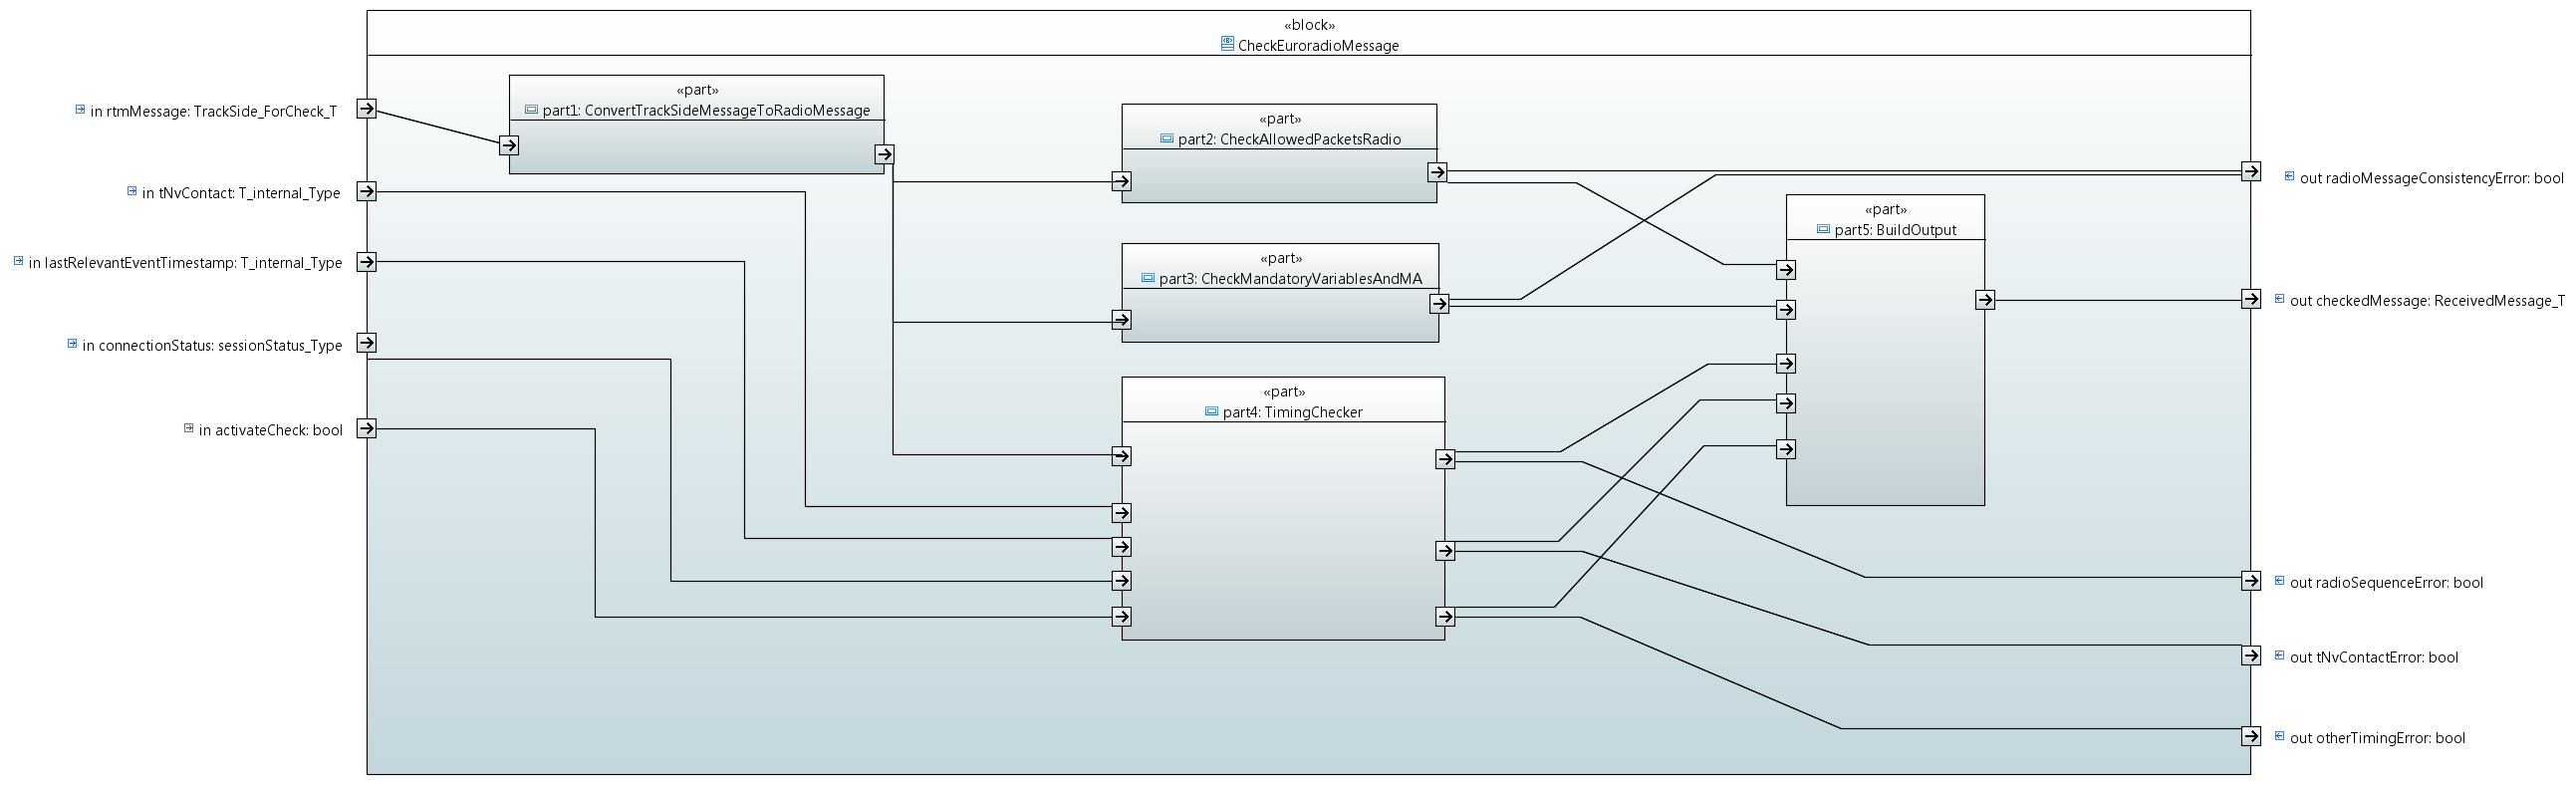
\includegraphics[width=\textwidth]{../images/CheckEuroradioMessage.png}
\caption{Component SysML diagram}\label{f:CheckEuroradioMessage_interface}
\end{figure}


\paragraph{Inputs}\label{s:CheckEuroradioMessage_inputs}

\subparagraph{rtmMessage}

\begin{longtable}{p{.25\textwidth}p{.7\textwidth}}
\toprule
Input name				& \verb rtmMessage \\
\midrule
Description				& Input message from API \\
\midrule
Source					& \verb Receive\_TrackSide\_Msg\_Pkg::Receive\_TrackSide\_Msg \\ 
\midrule
Type					& \verb Common_Types_Pkg::TrackSide_ForCheck_T \\
\midrule
Valid range of values	& n/a \\
\midrule
Behaviour when value is at boundary	& n/a \\
\midrule
Behaviour for values out of valid range	& n/a \\
\bottomrule
\end{longtable}

\subparagraph{tNvContact}

\begin{longtable}{p{.25\textwidth}p{.7\textwidth}}
\toprule
Input name				& tNvContact \\
\midrule
Description				& National value which defines the maximum time difference between a radio message or some defined special conditions. \\
\midrule
Source					& Current set of national values \\ 
\midrule
Type					& \verb Obu_BasicTypes_Pkg::T_internal_Type \\
\midrule
Valid range of values	& 0-255 \\
\midrule
Behaviour when value is at boundary & Message is always accepted (tNvContactError = false), see 7.5.1.148\\
\midrule
Behaviour for values out of valid range	& All messages are rejected (tNvContactError = true) \\
\bottomrule
\end{longtable}

\subparagraph{lastRelevantEventTimestamp}

\begin{longtable}{p{.25\textwidth}p{.7\textwidth}}
\toprule
Input name				& \verb lastRelevantEventTimestamp \\
\midrule
Description				& The input "lastRelevantTimestamp" is needed in order to check timeouts. In most of the cases, the timestamp of the last relevant event is the timestamp of the last message received. But the SRS defines special cases like driving through a defined radio hole. In this case, the timestamp of the last relevant event is the point of time, when the EVC has a radio connection again. \\
\midrule
Source					& Database \\ 
\midrule
Type					& \verb Obu_BasicTypes_Pkg::T_internal_Type \\
\midrule
Valid range of values	& dependent on hardware \\
\midrule
Behaviour when value is at boundary & n/a\\
\midrule
Behaviour for values out of valid range	& n/a \\
\bottomrule
\end{longtable}

\subparagraph{connectionStatus}

\begin{longtable}{p{.25\textwidth}p{.7\textwidth}}
\toprule
Input name				& \verb connectionStatus \\
\midrule
Description				& Status of the secure Euroradio session \\
\midrule
Source					& Management of Radio Communication \\ 
\midrule
Type					& \verb Radio_Types_Pkg::sessionStatus_Type \\
\midrule
Valid range of values &  \texttt{\{morc\_st\_inactive, morc\_st\_establishing, morc\_st\_maintaining, morc\_st\_terminating\}}\\
\midrule
Behaviour when value is at boundary & n/a\\
\midrule
Behaviour for values out of valid range	& n/a \\
\bottomrule
\end{longtable}

\subparagraph{activateCheck}

\begin{longtable}{p{.25\textwidth}p{.7\textwidth}}
\toprule
Input name				& \verb activateCheck \\
\midrule
Description				& If true, the Euroradio messages are checked, if false, the message is just passed without any modifications \\
\midrule
Source					& Debug settings \\ 
\midrule
Type					& \verb bool \\
\midrule
Valid range of values &  \texttt{\{true, false\}}\\
\midrule
Behaviour when value is at boundary & n/a\\
\midrule
Behaviour for values out of valid range	& n/a \\
\bottomrule
\end{longtable}

\paragraph{Outputs}\label{s:CheckEuroradioMessage_outputs}

\subparagraph{checkedMessage}

\begin{longtable}{p{.25\textwidth}p{.7\textwidth}}
\toprule
Output name				& \verb checkedMessage \\
\midrule
Description				& The message, which was checked with an updated valid flag. \\
\midrule
Destination				& ValidateDataDirection \\ 
\midrule
Type					& \verb Common_Types_Pkg::ReceivedMessage_T \\
\midrule
Valid range of values	& n/a \\
\bottomrule
\end{longtable}

\subparagraph{radioSequenceError}

\begin{longtable}{p{.25\textwidth}p{.7\textwidth}}
\toprule
Output name				& \verb radioSequenceError \\
\midrule
Description				& Indicates if the current message violated the sequence of radio messages. \\
\midrule
Destination				& \verb ProvidePositionReport \\ 
\midrule
Type					& \verb bool \\
\midrule
Valid range of values	& \texttt{\{true, false\}} \\
\bottomrule
\end{longtable}

\subparagraph{tNvContactError}

\begin{longtable}{p{.25\textwidth}p{.7\textwidth}}
\toprule
Output name				& \verb tNvContactError \\
\midrule
Description				& Indicates if a timeout on the radio channel occured.\\
\midrule
Destination				& \verb ProvidePositionReport \\ 
\midrule
Type					& \verb bool \\
\midrule
Valid range of values	& \texttt{\{true, false\}} \\
\bottomrule
\end{longtable}

\subparagraph{otherTimingError}

\begin{longtable}{p{.25\textwidth}p{.7\textwidth}}
\toprule
Output name				& \verb otherTimingError \\
\midrule
Description				& Indicates if other errors in the timing were detected, e.g. no last valid timestamp is available.\\
\midrule
Destination				& \verb ModeAndLevelManagement \\ 
\midrule
Type					& \verb bool \\
\midrule
Valid range of values	& \texttt{\{true, false\}} \\
\bottomrule
\end{longtable}

\subparagraph{radioMessageConsistencyError}

\begin{longtable}{p{.25\textwidth}p{.7\textwidth}}
\toprule
Output name				& \verb radioMessageConsistencyError \\
\midrule
Description				& Indicates, if a consistency error was detected in the Euroradio message. \\
\midrule
Destination				& EVC internal \\ 
\midrule
Type					& \verb bool \\
\midrule
Valid range of values	& \texttt{\{true, false\}} \\
\bottomrule
\end{longtable}

%% ---------- OLD -----------



\subsection{ValidateDataDirection in Manage\_TrackSideInformation\_Integration}

\subsubsection{Reference to the SRS or other Requirements (or other requirements)}
\begin{itemize}
 \item The functionality is mainly described in \cite[Chapter~3.6.3]{subset-026}.
\end{itemize}

\subsubsection{Short description of the functionality}
The operator will filter an input message in order to mark all elements as invalid, which are not designated for the current driving direction of the train.

\subsubsection{Interface}
The operator expects a message and information about the LRBG, passed balises and the current train position. As output, the message with packets valid for the current direction of driving is provided.

\subsubsection{Functional Design Description}
\begin{itemize}
 \item The operator contains two processing paths for different message types. Radio messages and balise group messages are handeled in a different way. For validating the data direction of a radio message, the check is performed using the balise group referenced in the radio message header as relevant balise group. For balise group message, the LRBG is used.
 \item The metadata of packets, which are recognized as not valid for the current driving direction, is invalidated.
\end{itemize}

\subsubsection{Reference to the Scade Model}
The SCADE model can be found on github under the following path: \url{https://github.com/openETCS/modeling/tree/master/model/Scade/System/ObuFunctions/ManageLocationRelatedInformation/BaliseGroup/ValidateDataDirection}

\subsection{InformationFilter}

\subsubsection{Reference to the SRS and other requirements}
\begin{itemize}
 \item The functionality of the InformationFilter is described in \cite[Chapter~4.8]{subset-026}.
\end{itemize}

\subsubsection{Short description of the functionality}
The function InformationFilter filters incoming information received
from Eurobalise, Euroradio, and Euroloop. The information is received
via messages and filtering is done depending on the criteria described
in \cite[Chapter~4.8]{subset-026}. Messages are only allowed to pass
the filter if specified critera are met like for example the correct
mode of the train (e.g. Full Supervision, Shunting, etc.) or the ETCS
level. Some messages have to be stored in a TransitionBuffer to be
later reevaluated by the filter again.

\subsubsection{Interface}
The interface of the information filter contains mainly the incoming
message and inputs to check for the conditions described in the
SRS. The complete interface is shown in table \ref{tbl:InformationFilterInterface}.

\begin{minipage}{\linewidth}
  \scriptsize
  \begin{tabular}{| l | l | l |}
    \hline
    \textbf{Name}                    & \textbf{Direction} & \textbf{Description}                                        \\ 
    \hline
    \texttt{inMessage}               & \texttt{IN}        & Received message that is valid for the train direction      \\
    \texttt{inLevel}                 & \texttt{IN}        & The current ETCS Level                                      \\
    \texttt{inMode}                  & \texttt{IN}        & The current train mode                                      \\
    \texttt{inSupervisingDevice}     & \texttt{IN}        & The device id which communicates with the current supervising
  RBC                                                                                                                   \\
    \texttt{inPendingL1Transition}   & \texttt{IN}        & Information if an ETCS Level 1 transition is pending        \\
    \texttt{inPendingL1L2Transition} & \texttt{IN}        & Information if an ETCS Level 2/3 transition is pending      \\
    \texttt{inPendingNTCTransition}  & \texttt{IN}        & Information if a NTC transition is pending                  \\
    \texttt{inPendingAckOfTrainData} & \texttt{IN}        & Information if the acknowledgement of train data is pending \\
    \texttt{inEmergencyBrakeActive}  & \texttt{IN}        & Information if the emergency brake is active                \\
    \texttt{inLastAckTextMessageId}  & \texttt{IN}        & The id of the last acknowledged message ID                  \\
    \texttt{inActiveCab}             & \texttt{IN}        & Information if the cab is active                            \\
    \texttt{inTrainDataValid}        & \texttt{IN}        & Information if the train data is valid                      \\
    \texttt{outMessage}              & \texttt{OUT}       & The filtered input message                                  \\
    \hline
  \end{tabular}
  \captionof{table}{Overview of the InformationFilter interface}
  \label{tbl:InformationFilterInterface}
\end{minipage}

\subsubsection{Functional Design Description}

\begin{figure}
\centering
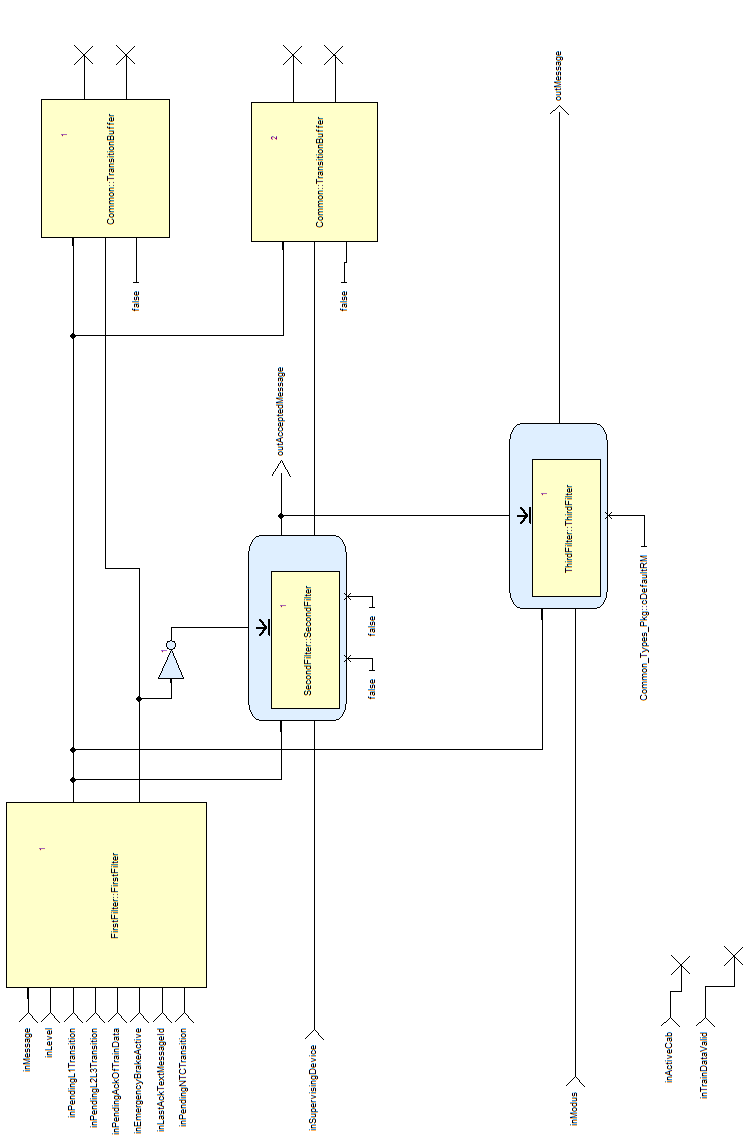
\includegraphics [width=\textwidth]{images/informationfilter-high-level-rot.png}
\caption{High level overview of the InformationFilter components.}
\label{fig:InformationFilterHighLevel}
\end{figure}

The filter receives track information (balise and radio) and filter
them depending of the mode, level and further information. Only
messages that pass the filter are valid and should be considered by
other ETCS subsystems. The figure \ref{fig:InformationFilterHighLevel}
show the high\-level decomposition of the functionality. The filter
functionality can be decomposed into a FirstFilter, SecondFilter,
ThirdFilter an TransitionBuffer.

\paragraph{FirstFilter} This filter performs filtering of messages
based on the current ETCS level. The decisions taken process is
described via a big decision table which contains rows for every
packet and columns for every ETCS level. This table encodes also if
certain additional information is necessary to filter a message like
pending ETCS Level transitions. Based on this filter packets of an
incoming message is either rejected, accepted or the whole message is
put in the TransitionBuffer. Messages are put in the TransitionBuffer
if there is an announced level transition and the received message is
only valid for the upcoming level.

\paragraph{SecondFilter} The SecondFilter mainly considers messages
that are received via Euroradio. Certain messages are directly
rejected while other may be stored in the TransitionBuffer. The buffer
is used to store messages that are received from non supervising RBCs,
but will be reevaluated after a RBC transition.

\paragraph{ThirdFilter} The last filter is functionally very similiar
the the FirstFilter, however it filters depending on the mode. It also
contains a decision table with rows for every packet but the columns
are modes.

\paragraph{TransitionBuffer} The InformationFilter uses two
TransitionBuffers. One is used to store up to three messages for the
ETCS level transition and the other buffer is used for RBC
transitions. The buffer is designed as a ring buffer and message are
read in FIFO order.

A detailed list of packages and their handling depending of ETCS level
or mode can be seen in table \ref{fig:PackagesListLevel} and
\ref{fig:PackagesListMode}.

\begin{figure}
\centering
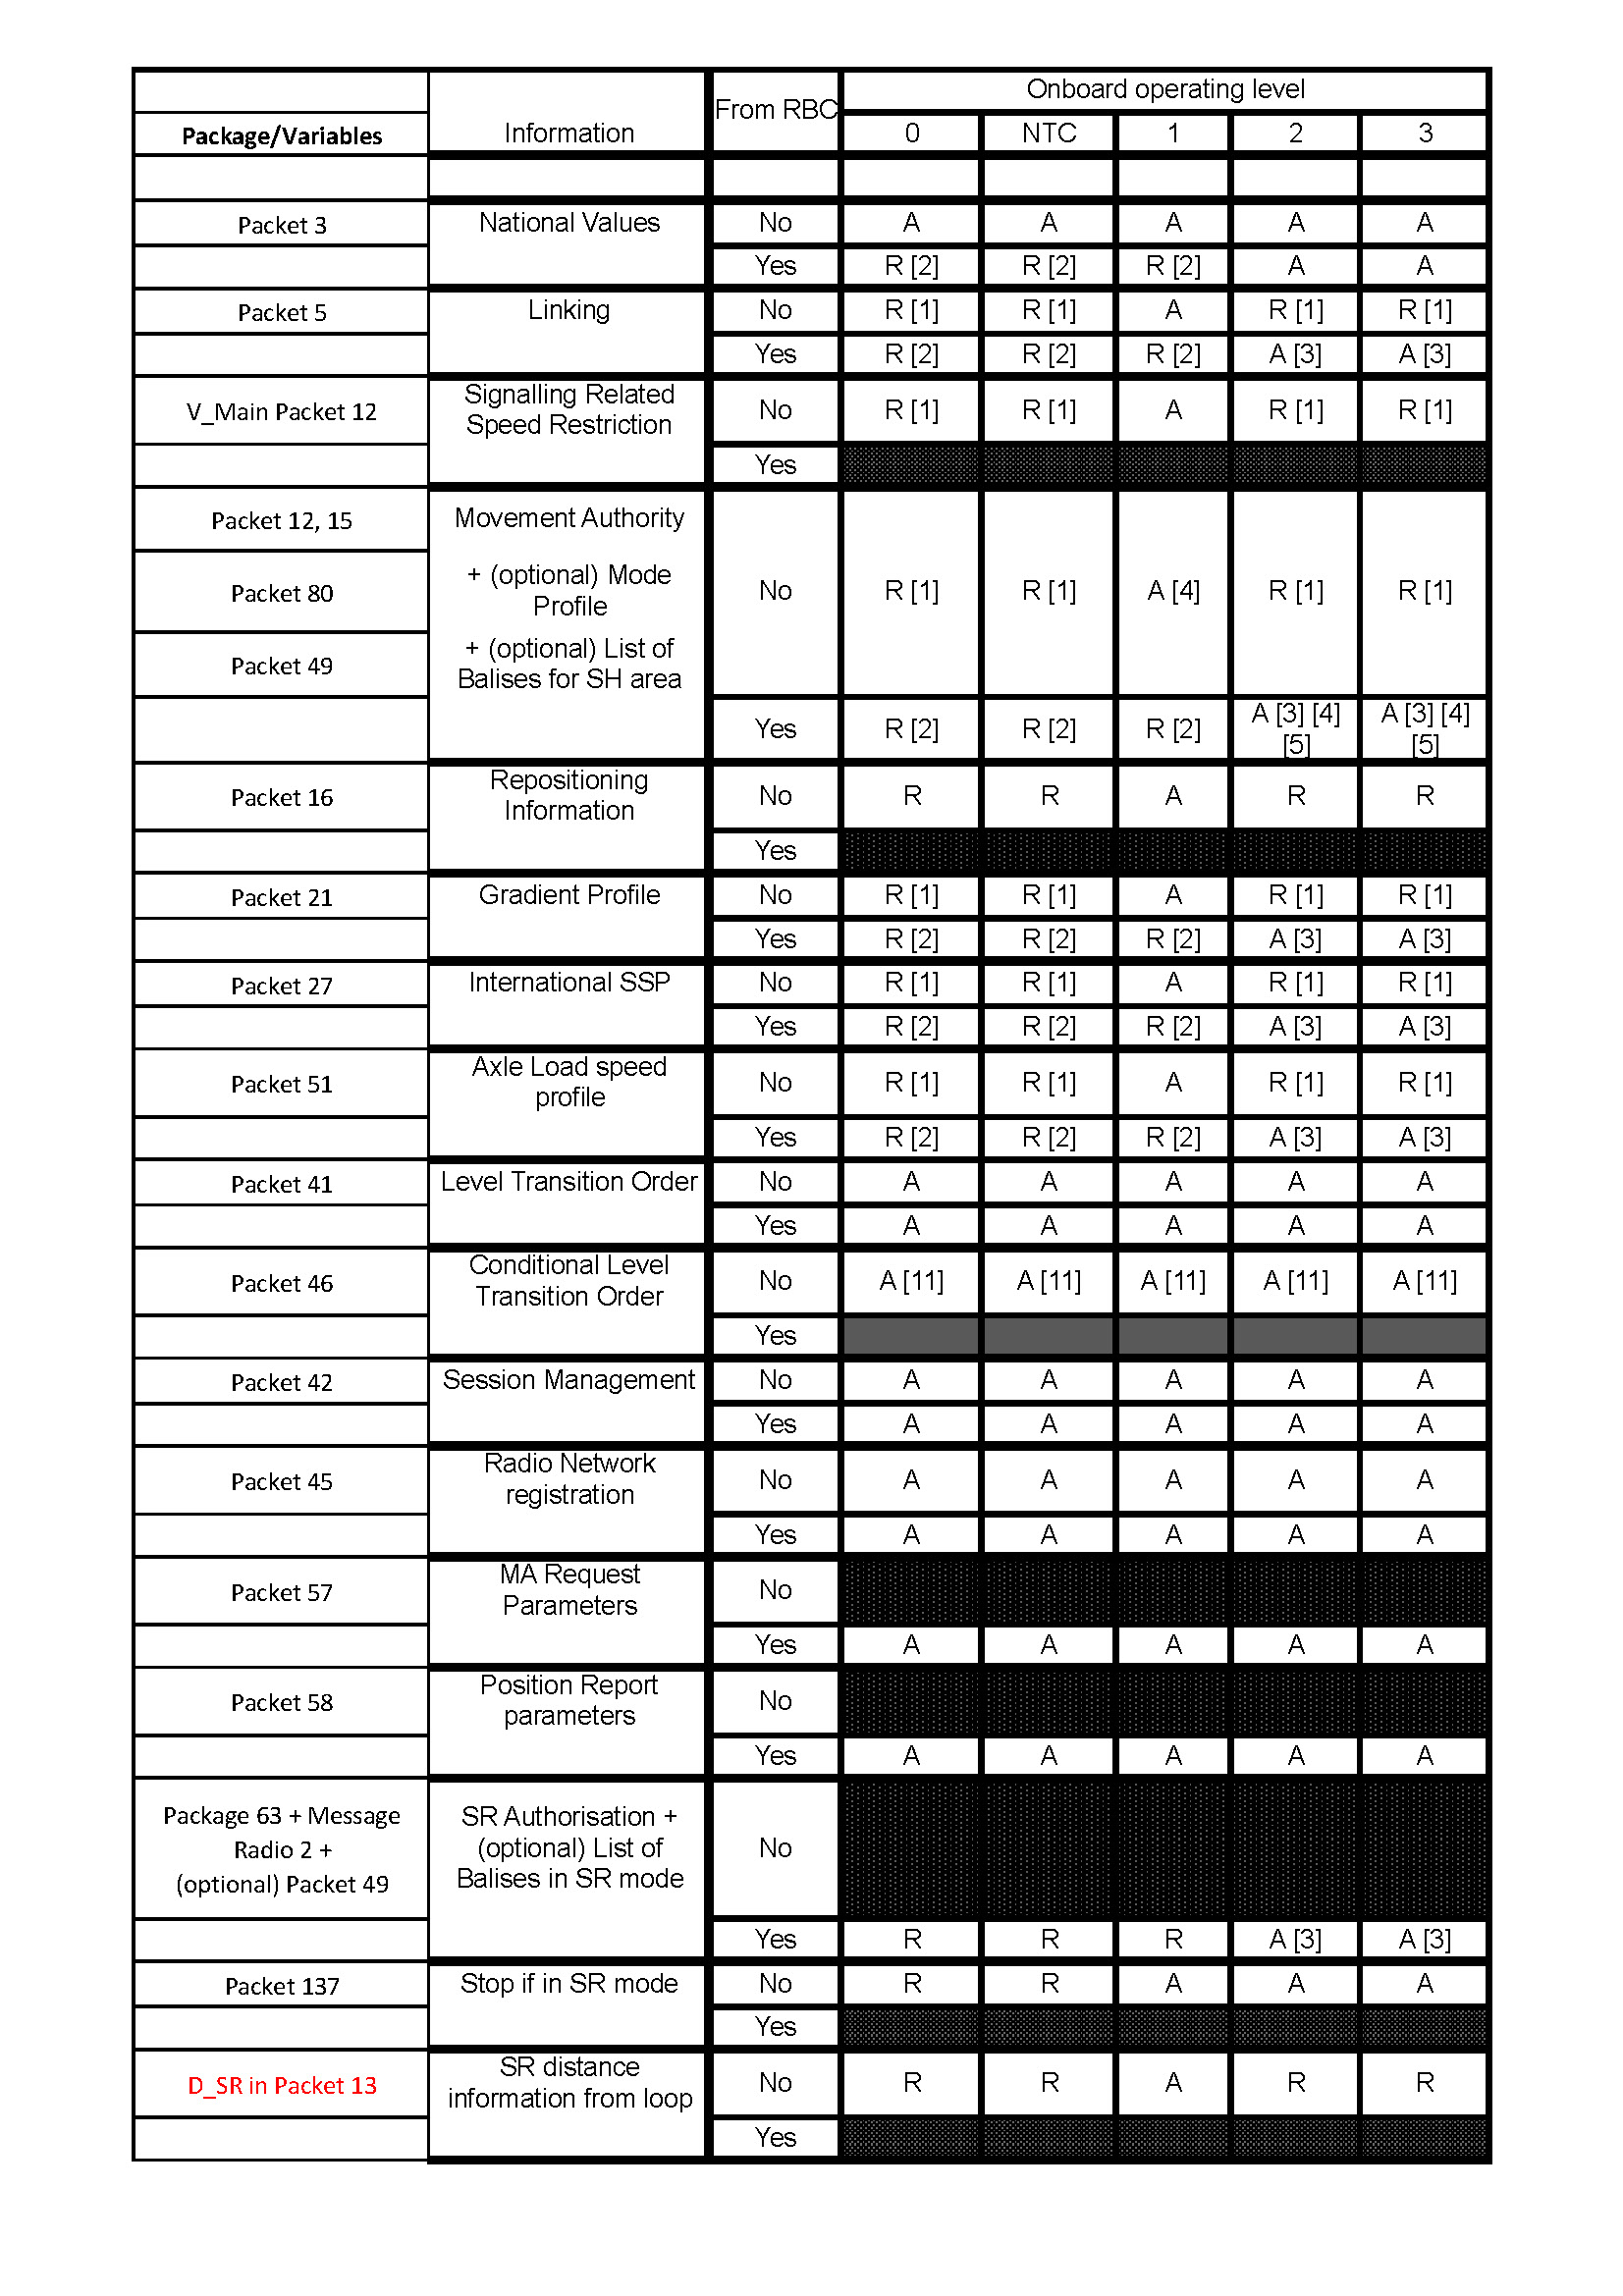
\includegraphics [scale=0.6]{images/LevelFilter1}
\end{figure}
\begin{figure}
\centering
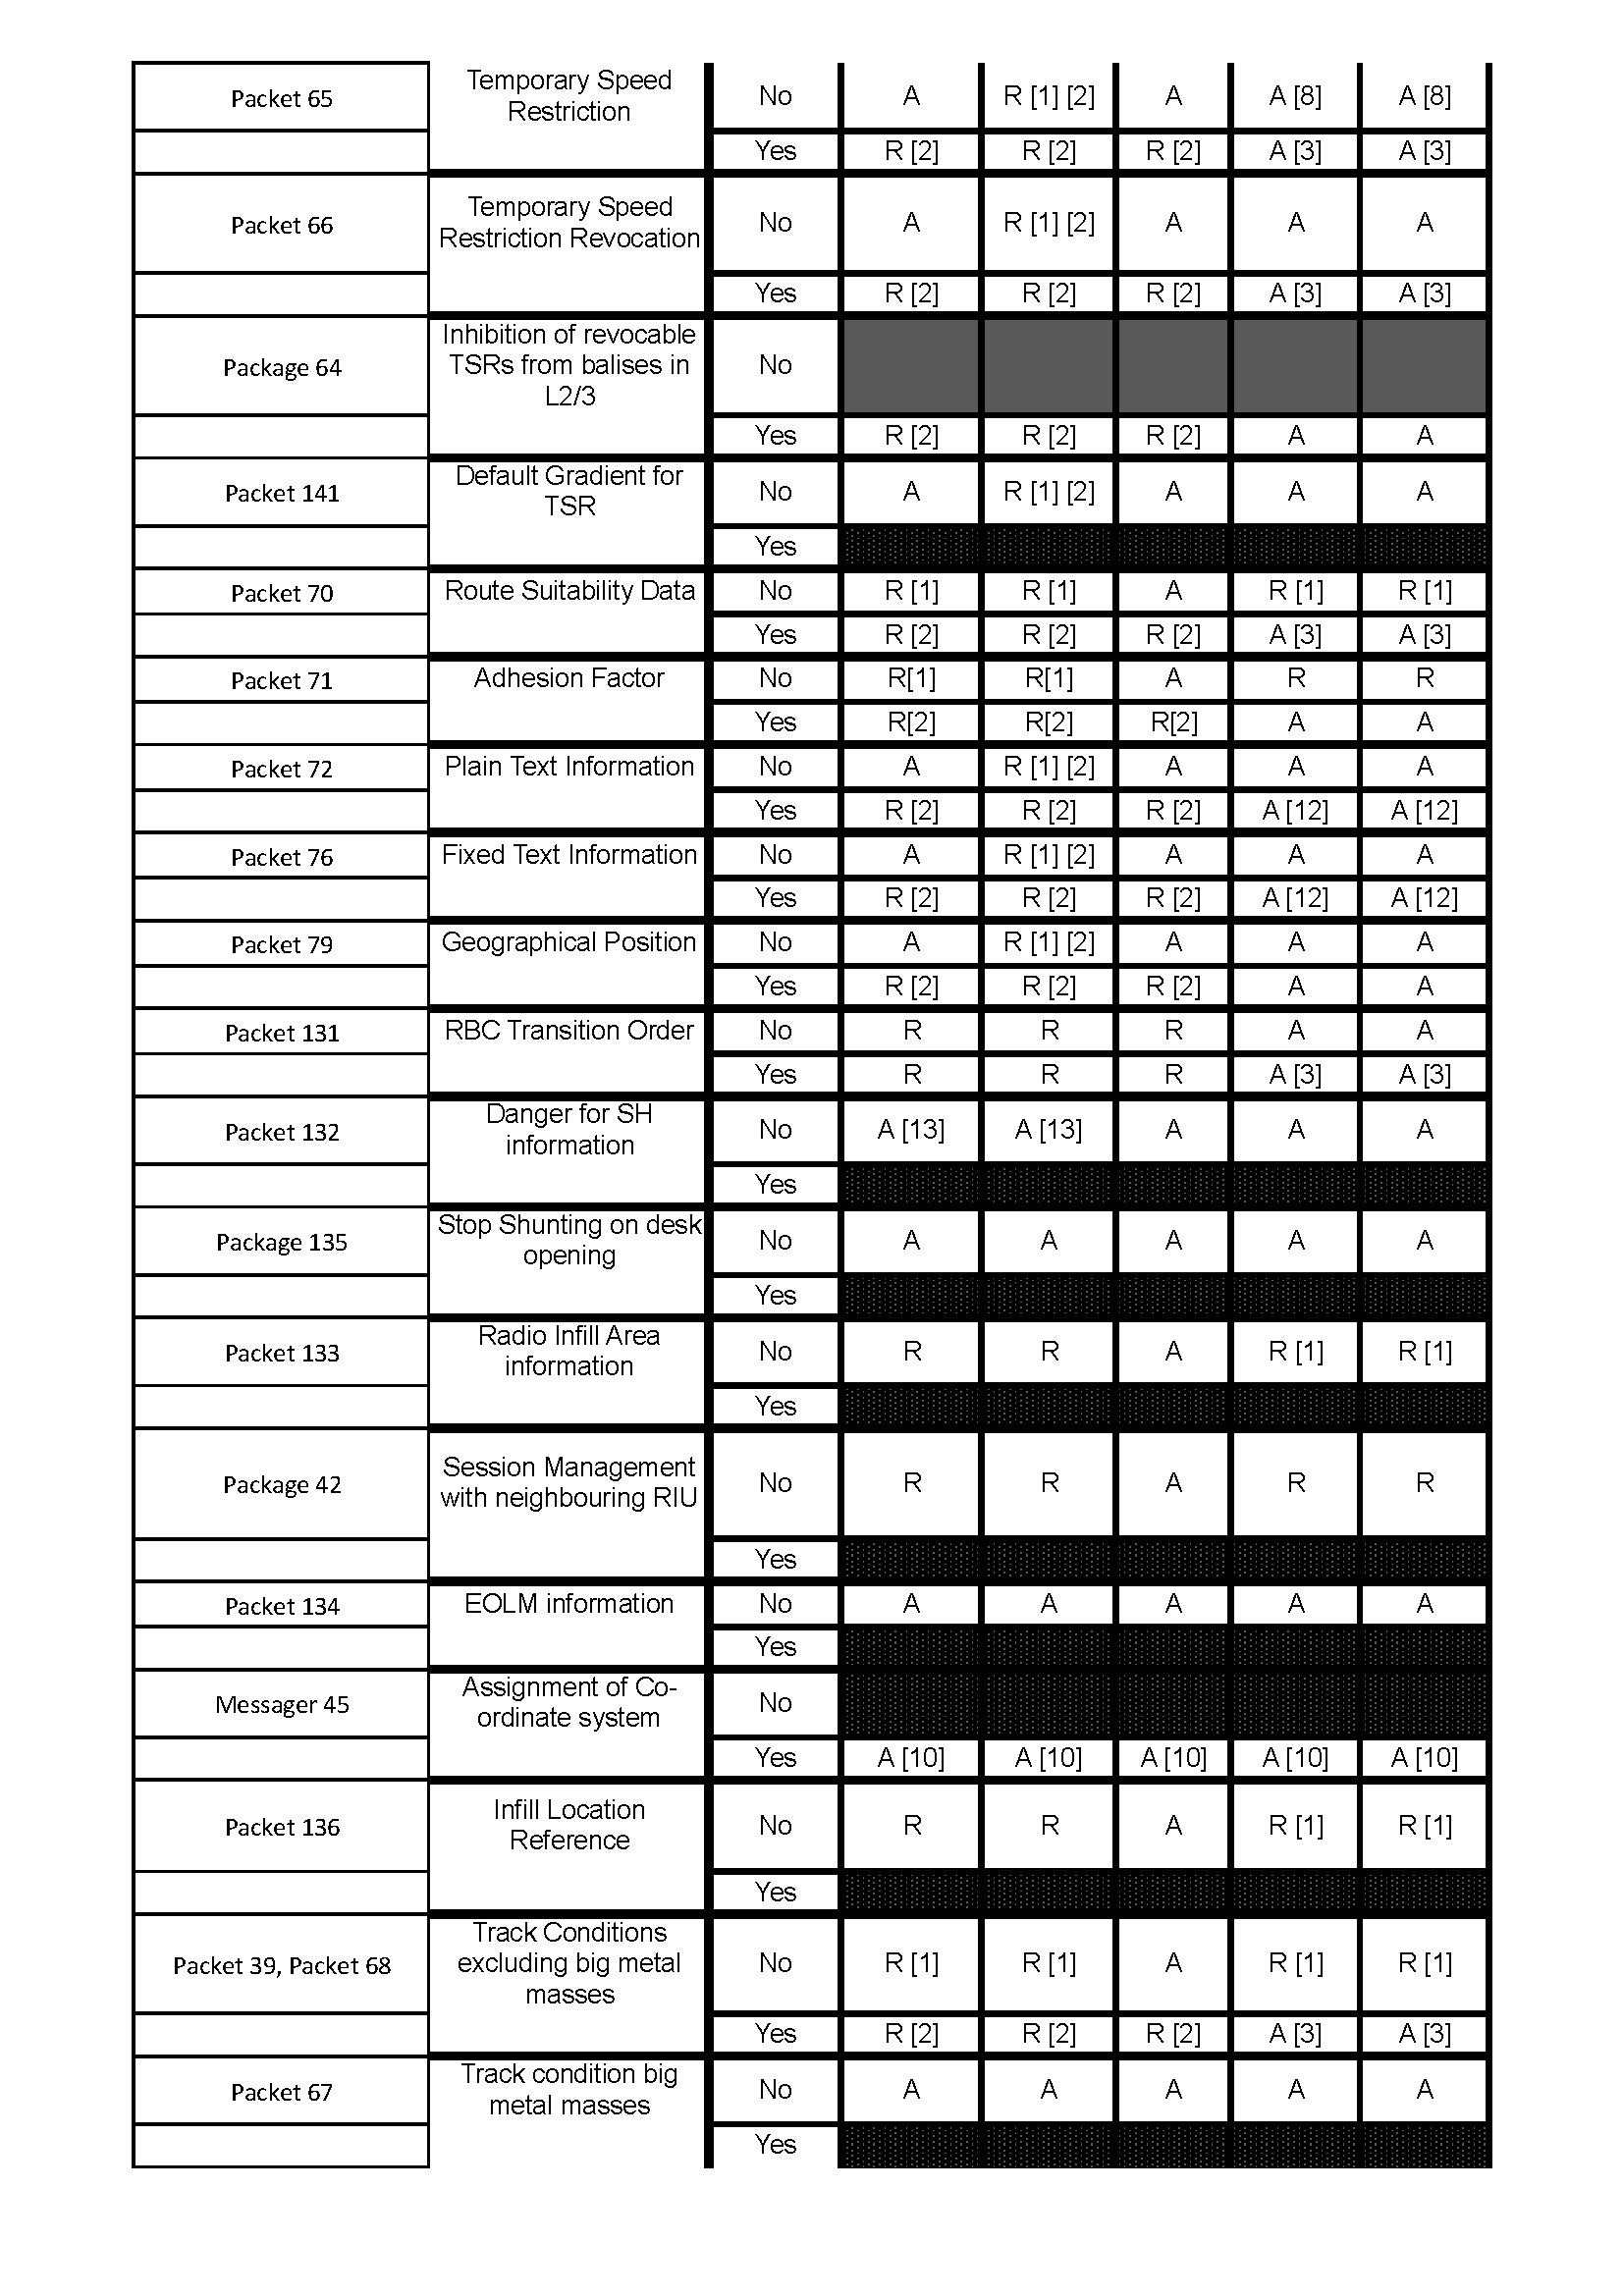
\includegraphics [scale=0.6]{images/LevelFilter2}
\end{figure}
\begin{figure}
\centering
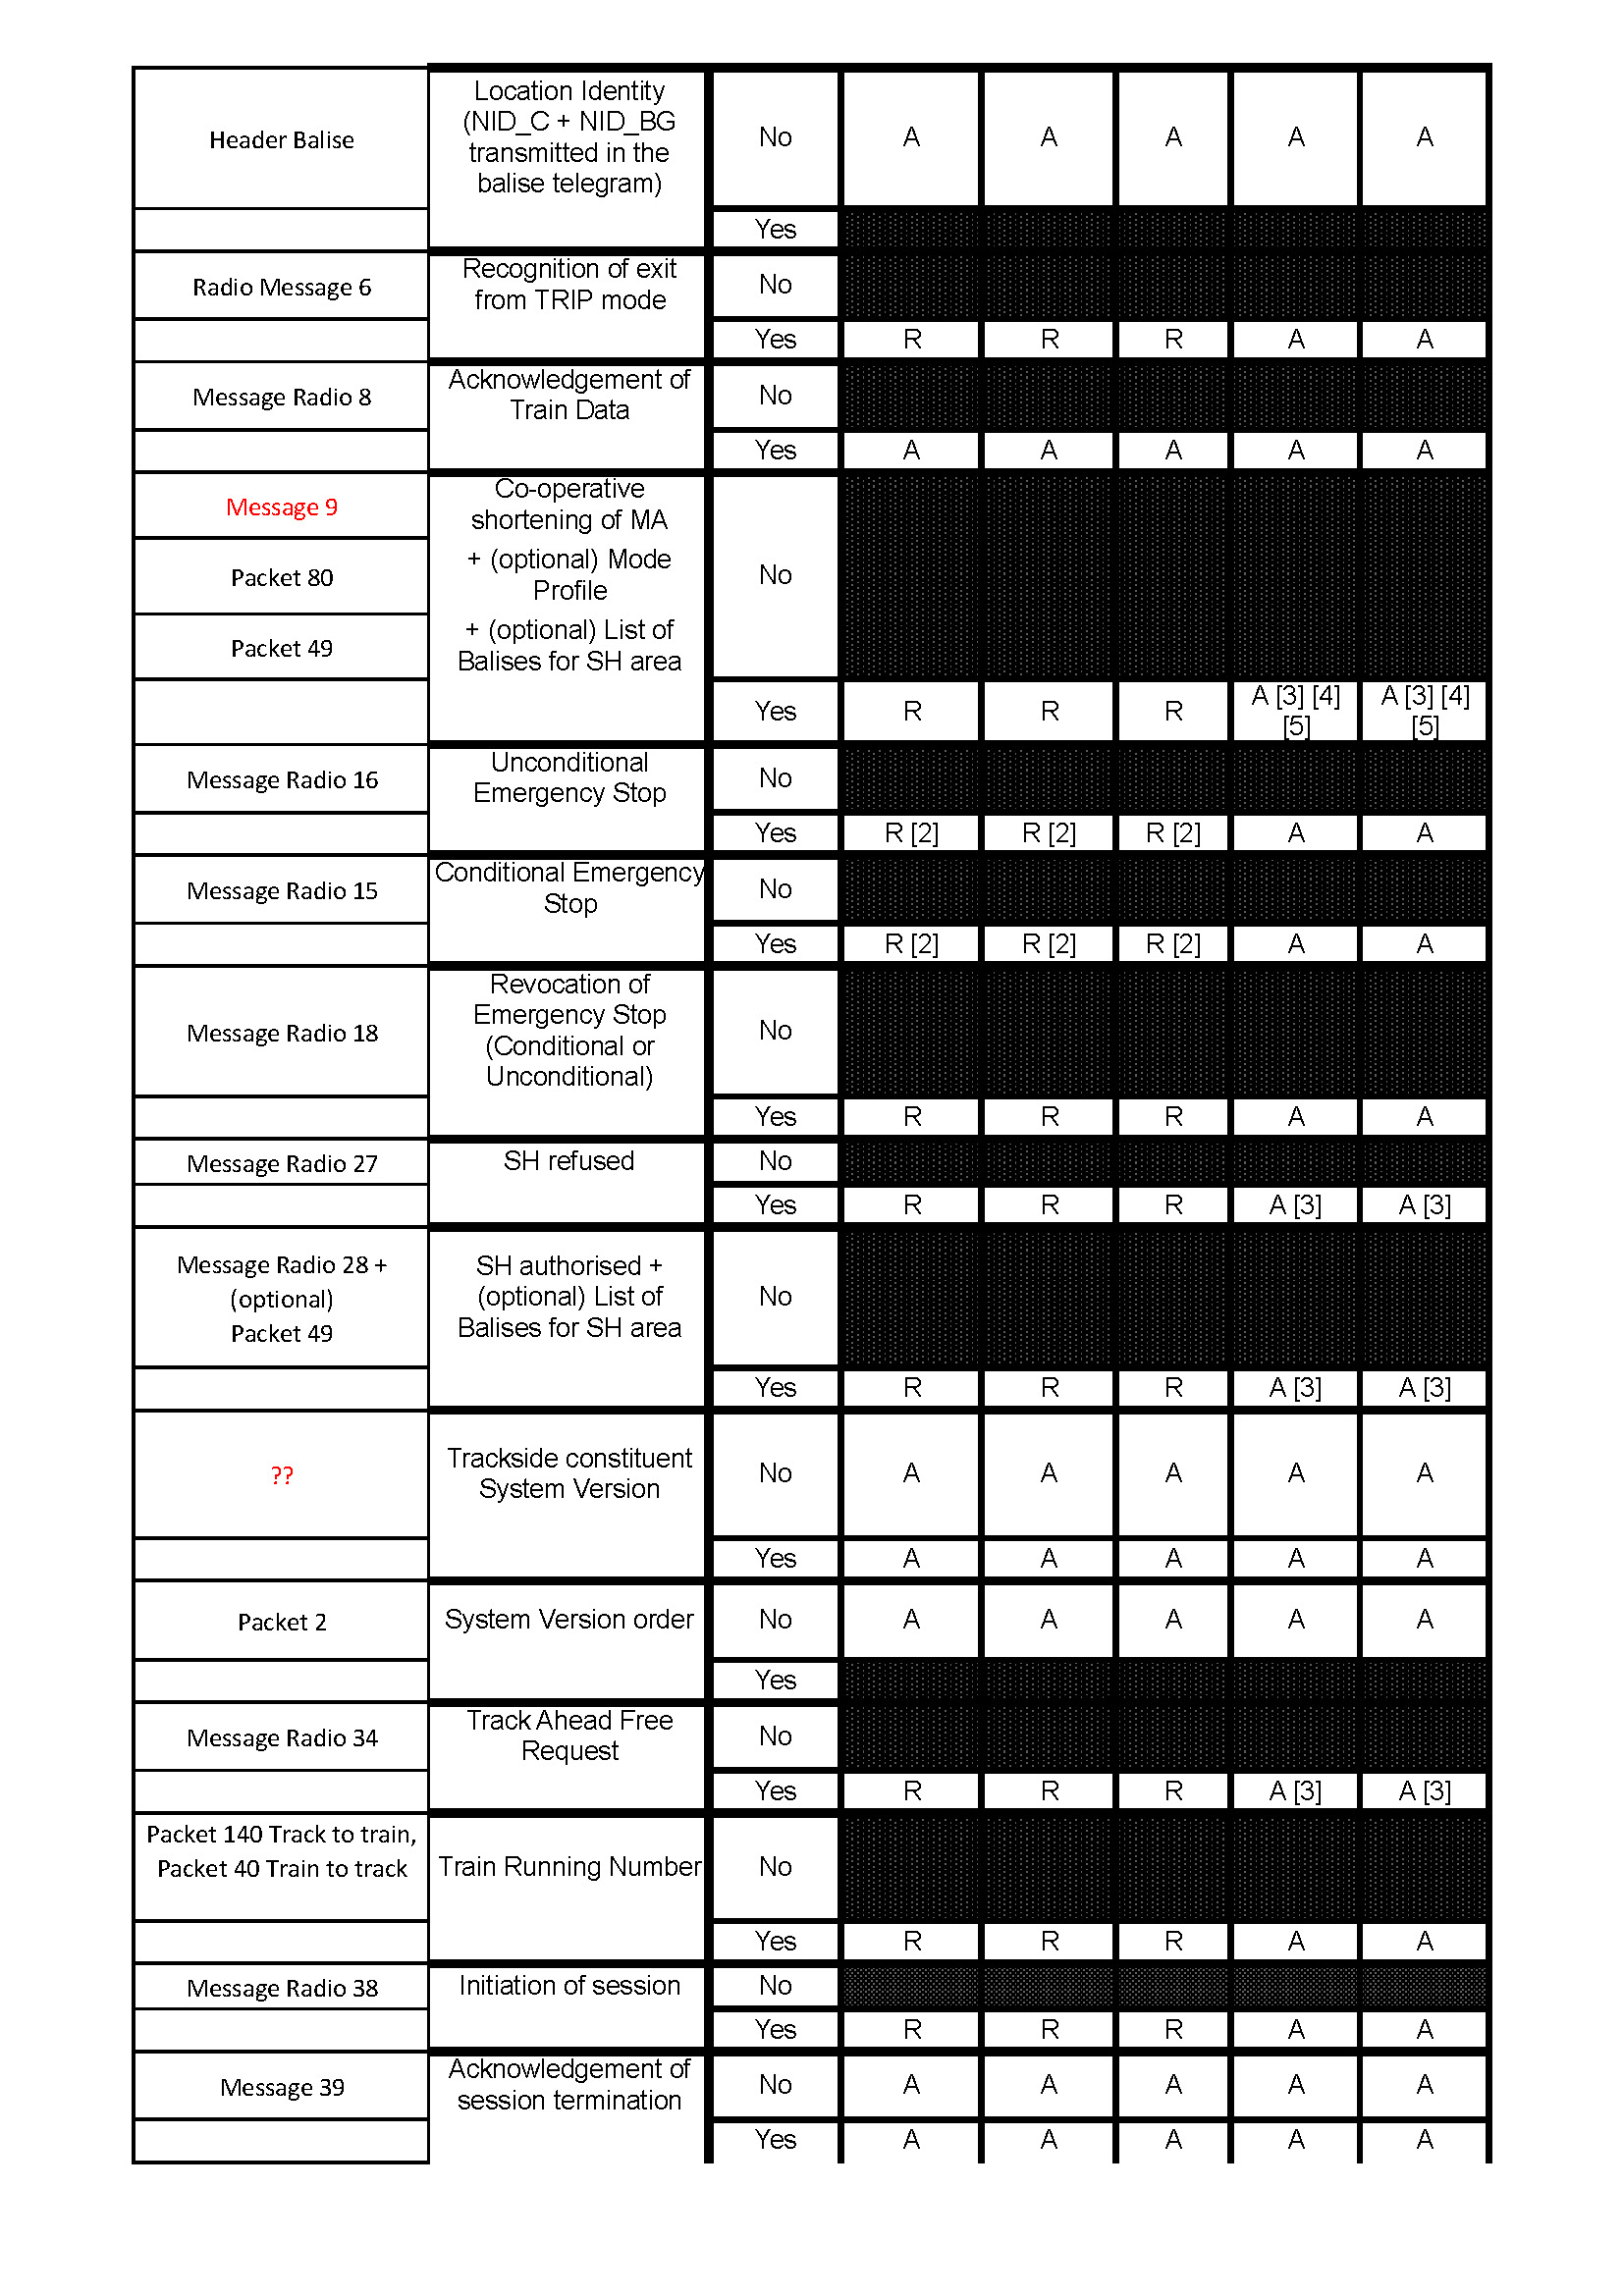
\includegraphics [scale=0.6]{images/LevelFilter3}
\end{figure}
\begin{figure}
\centering
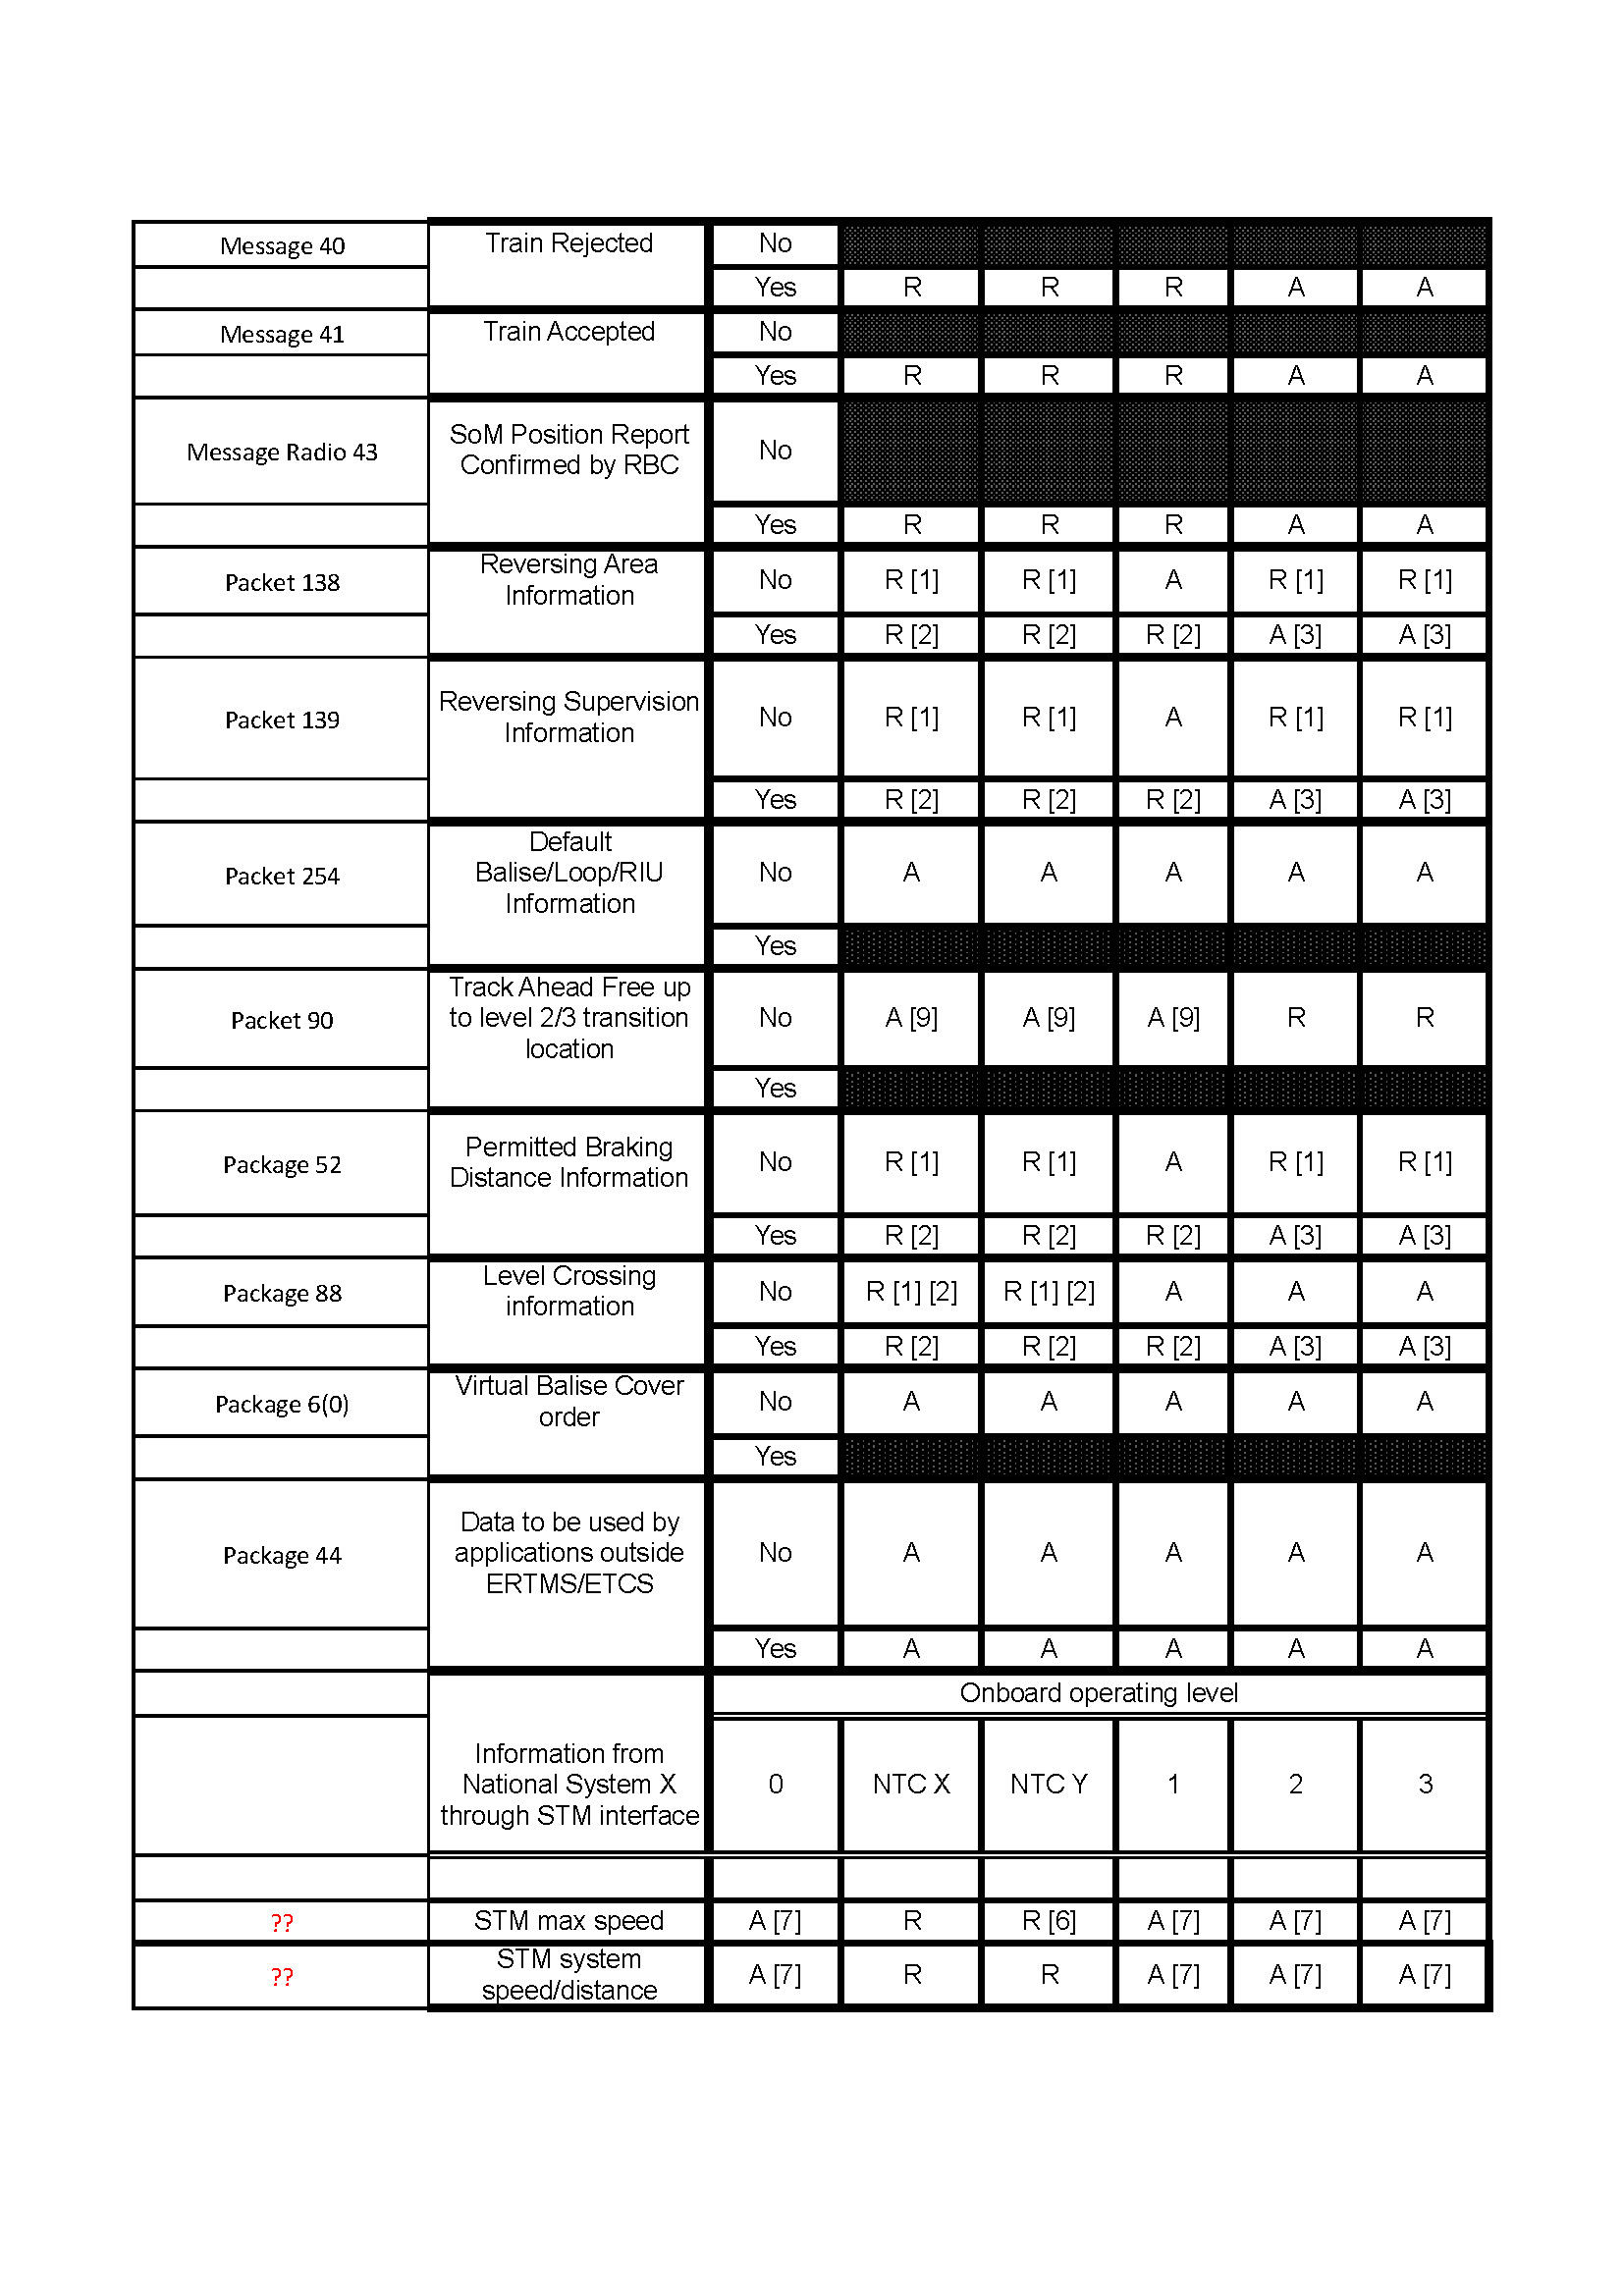
\includegraphics [scale=0.6]{images/LevelFilter4}
\caption{Lists of packages and their handling depending on train modes}
\label{fig:PackagesListLevel}
\end{figure}



\begin{figure}
\centering
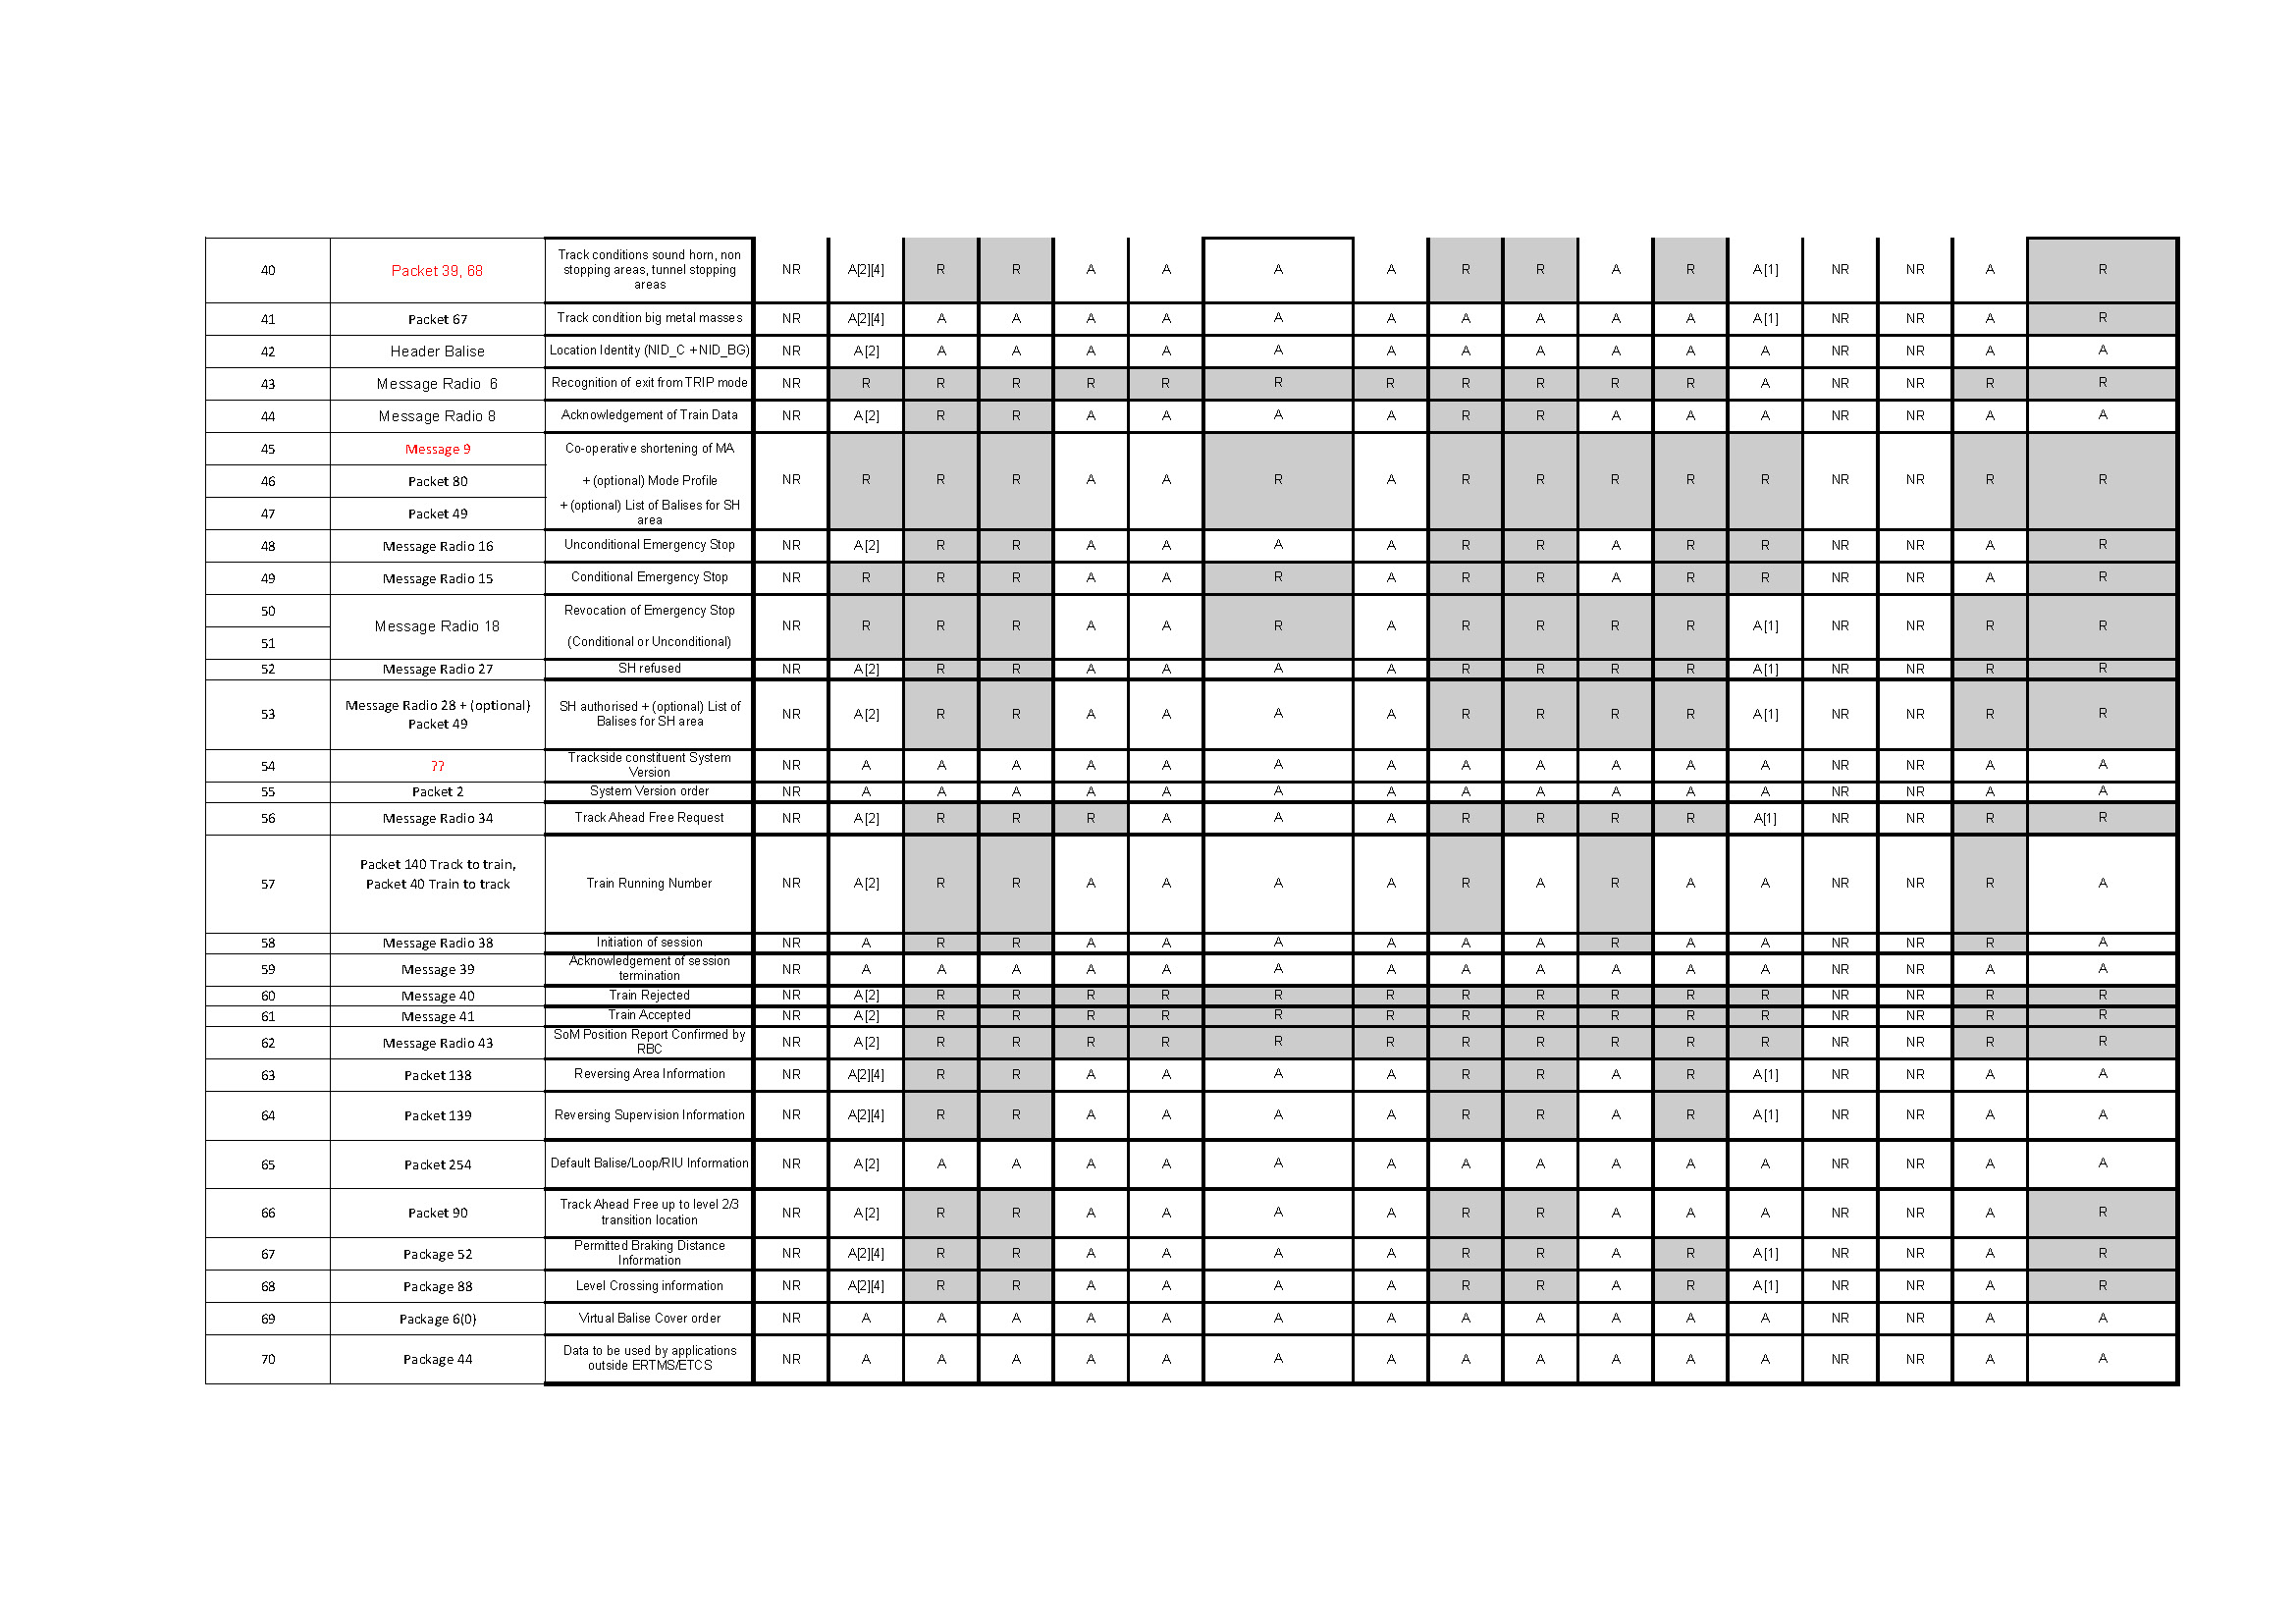
\includegraphics [angle=90, scale=0.8]{images/FilterMode1}
\end{figure}
\begin{figure}
\centering
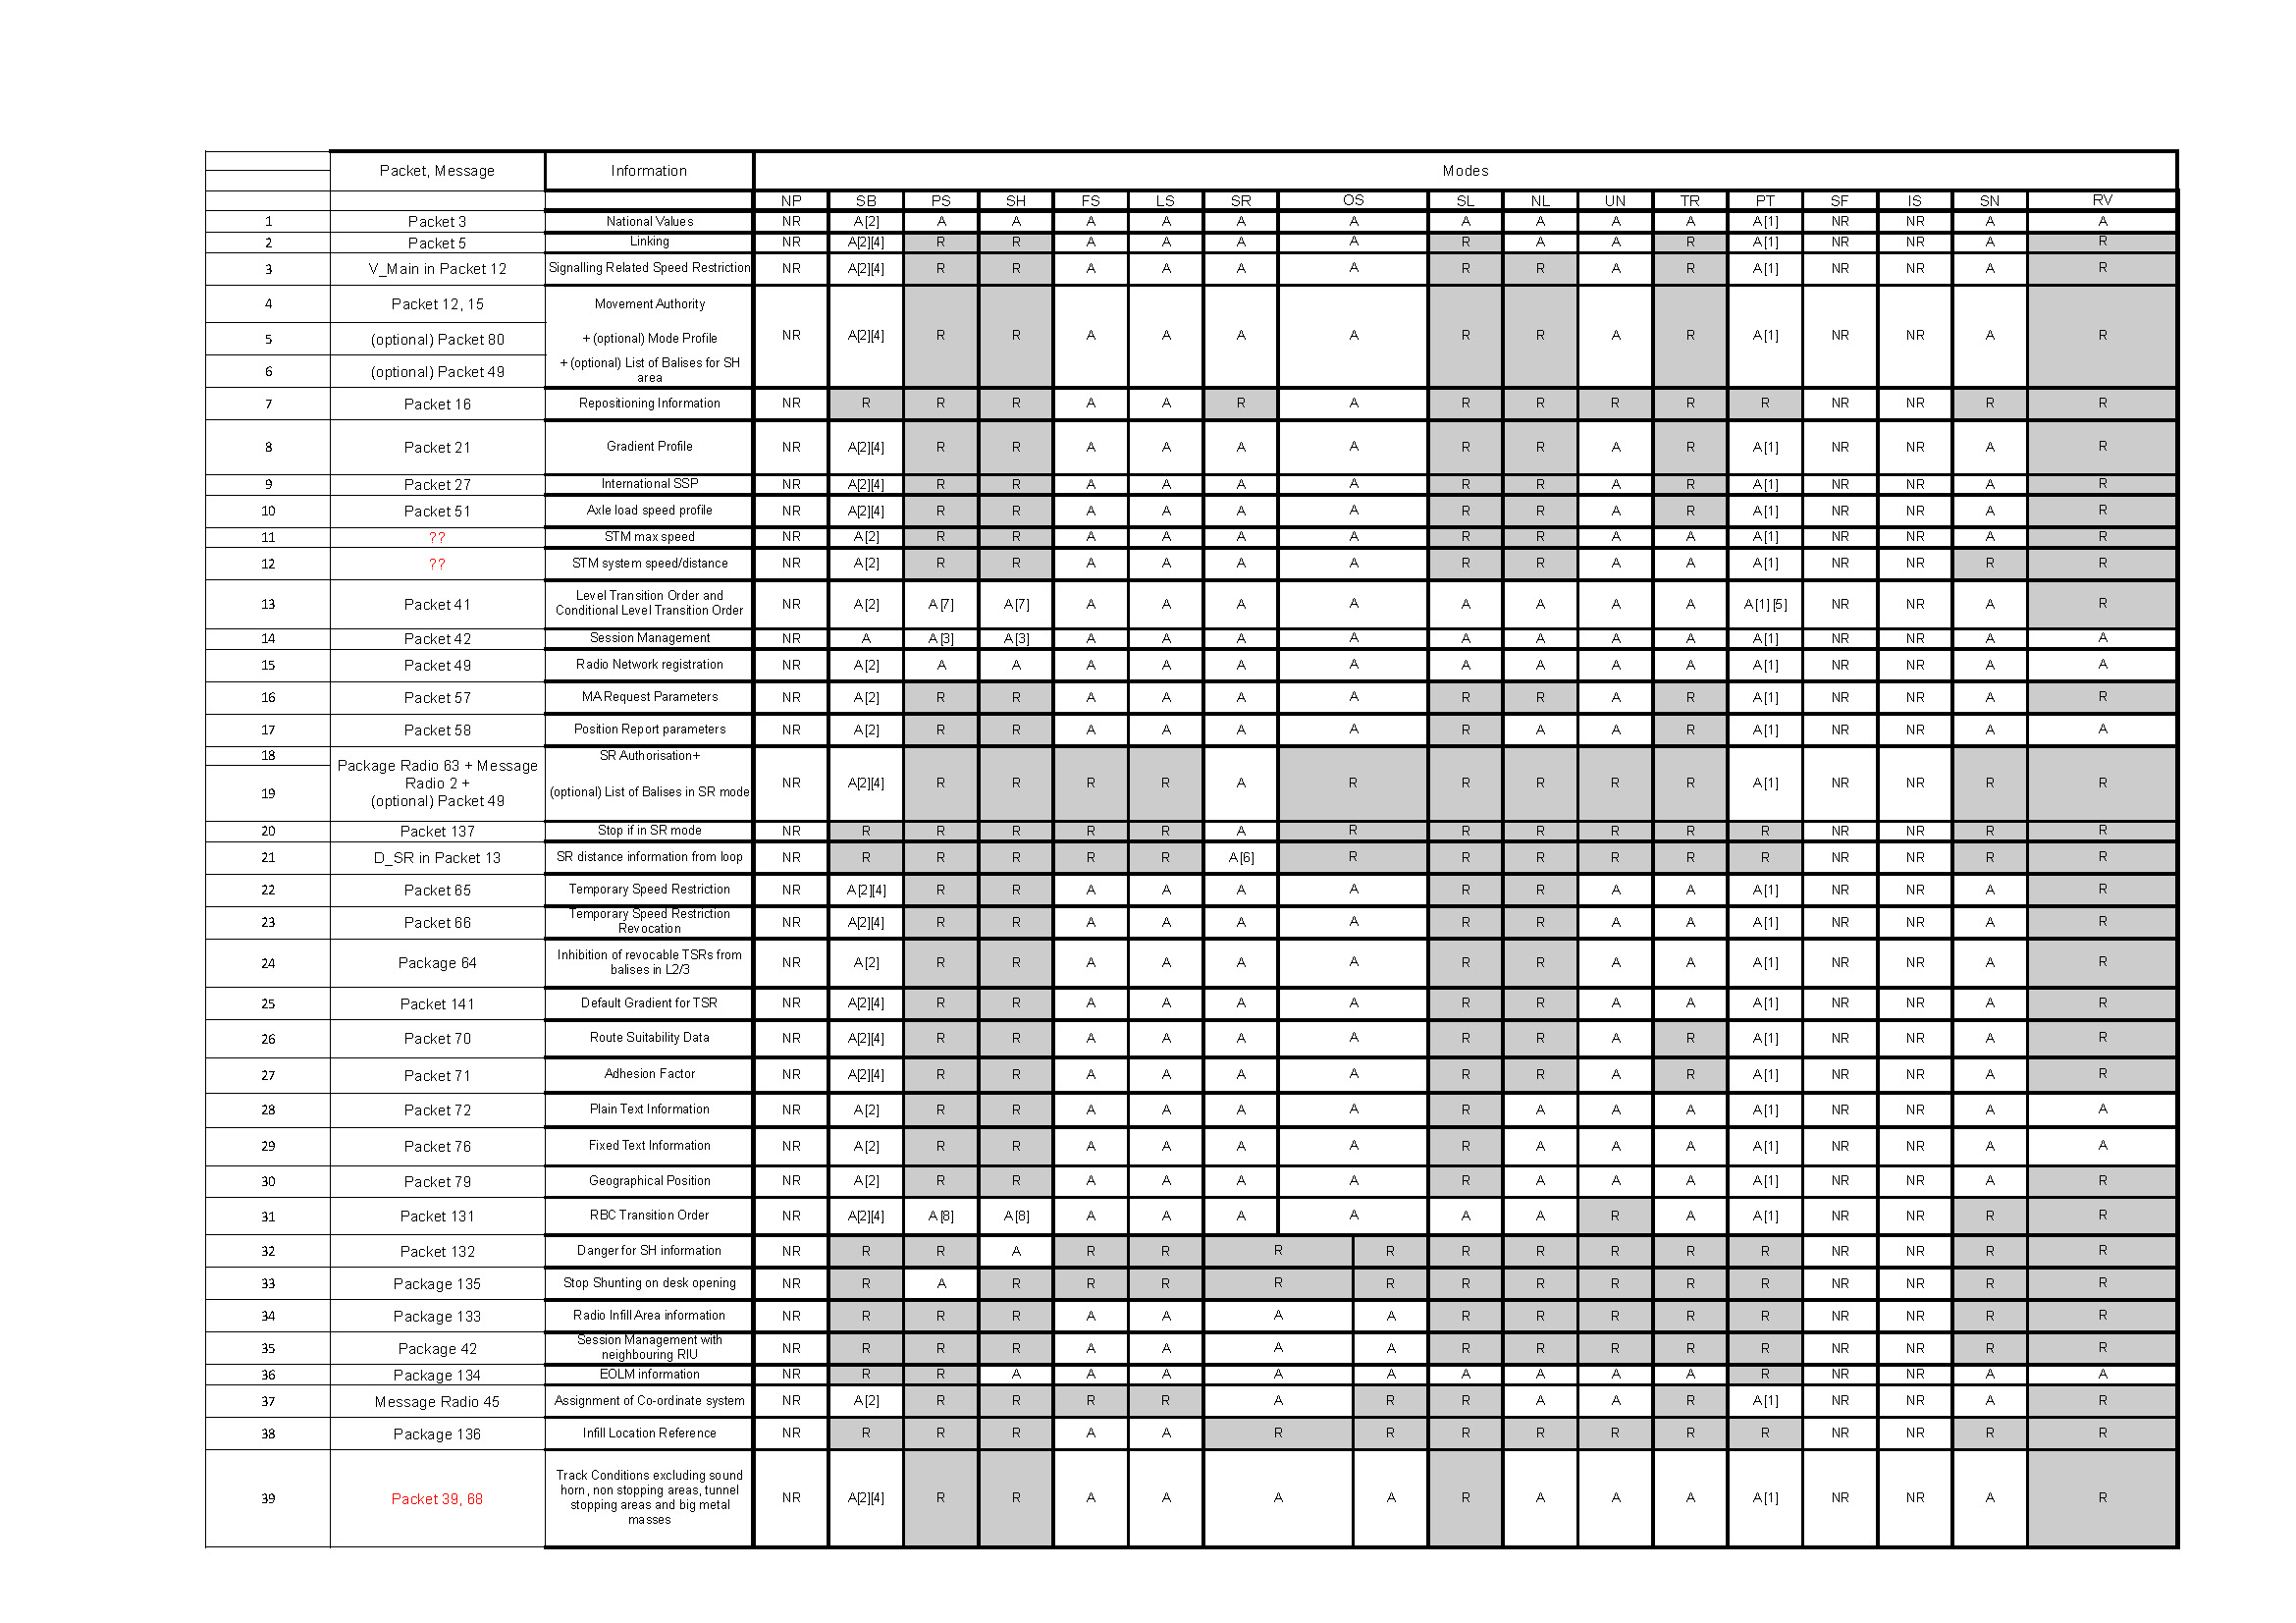
\includegraphics [angle=90, scale=0.8]{images/FilterMode2}
\caption{Lists of packages and their handling depending on train modes}
\label{fig:PackagesListMode}
\end{figure}

%%\subparagraph{Filtering (Mode/Level) - One packet per type}
%%\textbf{ISSUE: HOW MANY PKT 44, 65 AND 66 PER MESSAGE ARE MAXIMALLY SUPPORTED? (BH: who made this comment??)}\\

%% - Check on announced and immediate level transition orders in the messages to be filtered (needed for further criteria for filtering, to decide if the data shall be stored in the transition buffer).\\
%% - Filter data stored in the transition buffer according to the current level (what to do if similar information is available in the new message??). Data can be rejected, accepted or kept in the transition buffer.
%% (Filtering according to new level will be done directly afterwards in the next cycle)\\
%% - Filter new received messages according to the current level (new level will be done in the next cycle as according to \gls{SRS} data first has to be filtered according to old level and afterwards to new level). Data can be rejected, accepted or stored in the transition buffer.\\
%% - Filter (level) accepted data according to originating RBC (supervising or other). Information from \gls{BG}'s, loops or RIU is not filtered with this filter.\\
%% - Filter (level and RBC) accepted data according to the current mode (only reject or accept)\\


\subsubsection{Reference to the Scade Model}
The SCADE model can be found on github under the following path: \url{https://github.com/openETCS/modeling/tree/master/model/Scade/System/ObuFunctions/ManageLocationRelatedInformation/BaliseGroup/InformationFilter}
